\documentclass[12pt, hidelinks]{report}
\usepackage[table]{xcolor}

\usepackage[utf8]{inputenc}
\usepackage[italian]{babel}
\usepackage[T1]{fontenc}
\usepackage[a-1a]{pdfx}
\usepackage[pdfa]{hyperref}
\usepackage{bm}

\usepackage{lipsum}  

\usepackage{pdfpages}

\usepackage[a4paper]{geometry}
\usepackage{changepage}
\usepackage{tabularx}

\usepackage{amssymb, amsmath} %\usepackage{amssymb,amsmath,amsthm}
\usepackage{graphicx}
%\usepackage{url}
%\usepackage{hyperref}
%\usepackage{epsfig}
\usepackage{fancyhdr}
%\usepackage{setspace}
\usepackage{template}
\usepackage{listings}
\usepackage{rotating}

\usepackage{xcolor}

\usepackage{verbatim}

%New colors defined below
\definecolor{codegreen}{rgb}{0,0.6,0}
\definecolor{codegray}{rgb}{0.5,0.5,0.5}
\definecolor{codepurple}{rgb}{0.58,0,0.82}
\definecolor{backcolour}{rgb}{0.95,0.95,0.92}

%Code listing style named "codestyle"
\lstdefinestyle{codestyle}{
  backgroundcolor=\color{backcolour}, commentstyle=\color{codegreen},
  keywordstyle=\color{magenta},
  numberstyle=\tiny\color{codegray},
  stringstyle=\color{codepurple},
  basicstyle=\ttfamily\footnotesize,
  breakatwhitespace=false,         
  breaklines=true,                 
  captionpos=b,                    
  keepspaces=true,                 
  numbers=left,                    
  numbersep=5pt,                  
  showspaces=false,                
  showstringspaces=false,
  showtabs=false,                  
  tabsize=2
}

\lstset{style=codestyle}

%\usepackage{natbib}
%\usepackage{graphicx}
\usepackage{float}
\usepackage{multirow}
\usepackage{array}

\renewcommand{\arraystretch}{1.3}  % INTERLINEA
%\usepackage{caption}
\usepackage{subcaption}
\captionsetup{width=0.95\textwidth,font={small, sl},labelfont={bf}}
\usepackage[capitalise]{cleveref}
\crefname{figure}{Figura}{Figura}
\crefname{table}{Tabella}{Tabella}
\crefname{chapter}{Capitolo}{Capitolo}
%\addbibresource{biblio.bib}

\graphicspath{ {images/} }

% DATI STUDENTE e TESI
\newcommand{\myTitle}{Progettazione ed implementazione di un ambiente di emulazione di sistemi di edge computing e reti mobili 5G}
\newcommand{\myRefereeA}{Christian Quadri}
\newcommand{\myName}{Riccardo Carissimi}
\newcommand{\myMat}{962766}
\newcommand{\myYY}{2022-2023}
\newcommand{\dept}{Corso di Laurea in Informatica}

\begin{document}

\frontespizio

\begin{dedication}
A chi aiuta il prossimo col sorriso.
\\
A chi fa di tutto per essere la versione migliore di sé.
\\
A chi mi ha fatto sentire amato davvero.


\vspace{5mm}

A te che più di chiunque altro avresti voluto esserci.
\end{dedication}

\beforepreface
\afterpreface

\addcontentsline{toc}{chapter}{Introduzione}  
\chapter*{Introduzione}

%\section{Contesto e motivazioni}

L'evoluzione delle tecnologie di edge computing e delle reti mobili 5G sta rivoluzionando il panorama dell'elaborazione distribuita e dell'interconnessione delle risorse di calcolo. Queste tecnologie offrono una maggiore capacità di calcolo e connettività, consentendo l'esecuzione di applicazioni e servizi avanzati vicino ai dispositivi finali e riducendo la latenza nelle comunicazioni.

La comprensione del funzionamento e delle prestazioni di tali sistemi è fondamentale per garantire la progettazione e l'implementazione efficace di queste architetture. In particolare, l'ottimizzazione degli algoritmi di scheduling, responsabili della gestione delle risorse e del bilanciamento del carico, è cruciale per garantire prestazioni elevate e un utilizzo efficiente delle risorse disponibili.

L'uso di un ambiente di emulazione consente di analizzare il comportamento di applicazioni e sistemi complessi, permettendo di configurare la realtà in cui il sistema opera. L'adozione di questo approccio permette di studiare la reazione del sistema a cambiamenti del contesto, al fine di progettare sistemi sempre più sicuri e affidabili.

%\section{Obiettivi della tesi}

Questa tesi si propone di progettare ed implementare un ambiente di emulazione per reti 5G e sistemi di edge computing, analizzando inoltre i vari algoritmi di scheduling proposti per capirne le caratteristiche e valutarne l'impatto sull'architettura. 

Adotteremo l'approccio distribuito tramite il sistema di orchestrazione Kubernetes e garantiremo la scalabilità e la modellabilità dell'ambiente grazie al sistema di virtualizzazione Proxmox, basato su KVM. Grazie a questi strumenti mostreremo come abbiamo progettato un ambiente composto da più nodi di computazione e più punti di accesso, a cui gli utenti si collegano e richiedono l'applicazione.

Grazie alla flessibilità garantita dal sottosistema di virtualizzazione simuleremo la distanza geografica tra i nodi in modo da cambiare la realtà in cui l'ambiente opera. Per ogni algoritmo analizzeremo la reazione al cambiamento, ricavandone le peculiarità e riuscendo a proporre degli scenari in cui tale algoritmo ha prestazioni migliori.

%\section{Struttura della tesi}

Il lavoro di tesi è organizzato come segue:
\begin{description}
\item[Capitolo 1: Introduzione] In questo capitolo introduttivo, viene presentato il contesto delle tecnologie di edge computing e reti mobili 5G, e vengono descritti i motivi che hanno portato alla realizzazione di questa ricerca. Vengono inoltre esposti gli obiettivi della tesi e la sua struttura.
\item[Capitolo 2: Architettura degli orchestratori] Questo capitolo fornisce una panoramica dei concetti e dei fondamenti teorici alla base delle tecnologie di containerizzazione e orchestrazione. Verrà esaminato in particolare il sistema di Kubernetes.
\item[Capitolo 3: Progettazione] In questo capitolo mostreremo le scelte progettuali intraprese nella realizzazione del sistema di emulazione. Analizzeremo anche le possibili anomalie che si possono presentare e mostreremo come reagisce il sistema.
\item[Capitolo 4: Implementazione] Nell'implementazione renderemo esplicite le scelte implementative e le motivazioni di queste. Parleremo di Kubernetes e Proxmox e della come sono state degradate le performance di rete.
\item[Capitolo 5: Analisi dei risultati] In questo capitolo vengono presentati e analizzati i risultati ottenuti attraverso l'esperimento di emulazione. Vengono confrontate le prestazioni dei diversi algoritmi di scheduling e vengono valutate le loro caratteristiche.
\item[Capitolo 6: Conclusioni] Nelle conclusioni vengono riassunti i principali risultati ottenuti e vengono fornite raccomandazioni per la scelta dell'algoritmo di scheduling più adatto. Vengono inoltre proposte possibili direzioni future di ricerca.
\end{description}

% \section{Sintesi}

% Questa introduzione ha fornito un contesto sulle tecnologie di edge computing e reti mobili 5G, evidenziando l'importanza degli algoritmi di scheduling per l'efficienza e le prestazioni dei sistemi di edge computing. Gli obiettivi della tesi sono stati presentati, insieme alla struttura generale del lavoro. Nel prossimo capitolo, verranno forniti i fondamenti teorici necessari per comprendere appieno il contesto di questa ricerca.

\addcontentsline{toc}{chapter}{Architettura degli orchestratori}  
\chapter{Architettura degli orchestratori}

%\section{Introduzione}
Kubernetes è un sistema open-source per l'orchestrazione  di container comunemente abbreviato con la sigla "K8s", sviluppato da Google nel 2014. È stato progettato per automatizzare il deployment, la scalabilità e la gestione di applicazioni containerizzare su cluster di host.

Kubernetes è stato adottato da molte grandi aziende e provider di servizi cloud, è lo standard \textit{de facto} per l'orchestrazione di container ed è supportato da un vastissimo ecosistema di strumenti e servizi complementari che fanno di questo strumento il proprio core.

\section{Background sui container}
\subsection{Cosa sono i container}
I container sono una tecnologia di virtualizzazione che permette di eliminare il mantra riassumibile con la frase "It works on my machine".
Il mondo dello sviluppo software ha per anni dovuto fare i conti con una parte di deployment dei servizi difficoltosa. In un ambiente tradizionale, infatti, è necessario installare le dipendenze (della versione corretta), configurarle ed eventualmente anche gestire più versioni installate contemporaneamente.

L'esplosione dell'approccio DevOps attribuisce agli sviluppatori la gestione della parte di \textit{operations} dove i container sono la tecnologia chiave: permettono la creazione di applicazioni e la gestione del sistema che le circonda.
Per creare e gestire i container sono disponibili diverse tecnologie: una delle più popolari è Docker.

\subsection{Perché containerizzare}
Come evidenziato in \figurename~\ref{fig:container_vs_vm}, containerizzare ha molti vantaggi, che sono molto simili a quelli delle macchine virtuali (VM) a differenza delle quali utilizzano la funzionalità di isolamento del kernel del sistema operativo host per creare un ambiente isolato che rende i container più leggeri ed efficienti delle VM.

Questo risparmio non solo permette di sfruttare maggiormente l'hardware a disposizione ma consente anche un cambio di paradigma: un'applicazione non è più monolitica ma composta da più componenti indipendenti che possono essere scalati orizzontalmente a piacere.

\begin{figure}[h]
    \centering
    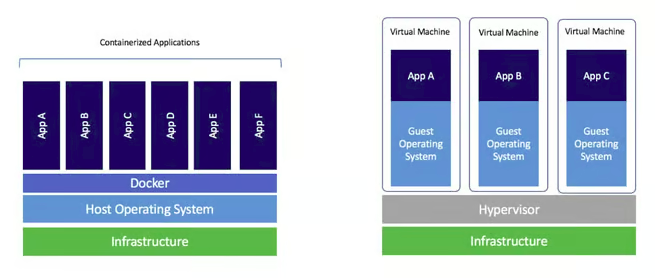
\includegraphics[width=\linewidth]{1_container_vs_vm.png}
    \caption{Comparazione tra lo schema di un container e quello di una VM \cite{container_vs_vm}}
    \label{fig:container_vs_vm}
\end{figure}

\subsection{Perché orchestrare i container}
Orchestrare i container permette di gestirne e coordinarne l'attività per sfruttare i diversi vantaggi che derivano, che elenchiamo di seguito:
\begin{itemize}
    \item deployment semplificato: l'orchestrazione semplifica molto la fase di deployment e la rende meno suscettibile ad errori umani in quanto ne automatizza il processo. 
    \item scalabilità: un altro vantaggio è sicuramente la possibilità di scalare \textit{on the fly} il numero di container in base a regole predeterminate. Questo vantaggio permette di fornire all'utente un servizio reattivo senza sprecare risorse nei momenti di traffico meno intenso.
    \item gestione delle risorse: è possibile inoltre limitare o garantire delle risorse a specifici container o servizi permettendo di evitare che un servizio obblighi gli altri a offrire performance peggiori.
    \item bilanciamento del carico: è possibile bilanciare il carico tra più host per non sovraccaricare una singola macchina e offrire delle \textit{performance} equiparabili nonostante il servizio sia hostato su server eterogenei.
    \item gestione dello stato e ripristino: infine è possibile gestire lo stato di un servizio ed eventualmente ripristinare l'operatività dei container in modo automatico al fine di aumentare di molto l'affidabilità del servizio e diminuire le interruzioni.
\end{itemize}

\section{Struttura di Kubernetes}

\subsection{L'architettura generale}
Kubernetes è composto da più nodi che corrispondono a una macchina (virtuale o fisica) che può eseguire i servizi. 
Esistono due categorie:
\begin{itemize}
    \item control plane, ovvero il nodo che si occupa di gestire il cluster, di cui vedremo le varie componenti. In generale si occupa di gestire il deployment dei container sui vari nodi worker. Siccome la sua \textit{availability} è vitale per la vitalità del cluster spesso sono disponibili più nodi \textit{control plane} di backup, in configurazione \textit{high availability} (HA). Di questi nodi ne può essere attivo solo uno, che gestirà il cluster mentre gli altri nodi subentreranno solo se necessario.
    \item worker: sono i nodi che eseguono i container, gestiti dal nodo \textit{control plane}. La loro disponibilità non è vitale in quanto sono facilmente rimpiazzabili, deployando di conseguenza i container sugli altri nodi.
\end{itemize}

In \figurename~\ref{fig:kubernetes-general-architecture} è possibile osservare l'architettura generale di un cluster Kubernetes.

\begin{sidewaysfigure}[h]
    \centering
    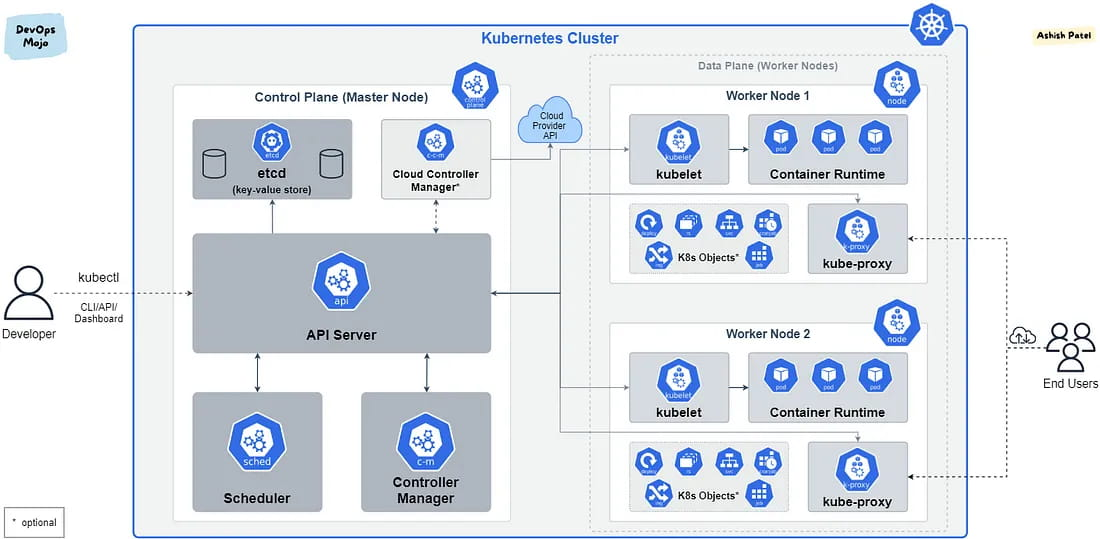
\includegraphics[width=\linewidth]{2_kubernetes_general_architecture.jpg}
    \caption{Schema generale di un cluster di Kubernetes \cite{kubernetes_architecture}}
    \label{fig:kubernetes-general-architecture}
\end{sidewaysfigure}

\subsection{I nodi \textit{worker}}
I nodi \textit{worker}, anche chiamati \textit{compute nodes}, sono formati da vari componenti che ne permettono il funzionamento. 

Prima di elencare i componenti dobbiamo descrivere i \textit{Pod}, cioè le più piccole unità di calcolo che si possono creare e gestire in Kubernetes. Consistono in un gruppo di uno o più container, con risorse di rete e storage condivise i cui contenuti sono sempre co-localizzati e co-schedulati. Per lo scopo del nostro progetto possiamo pensare a un \textit{Pod} come a un container. 

Ora possiamo descrivere i componenti principali della struttura dei nodi \textit{worker}:

\begin{itemize}
    \item kubelet: è un \textit{agent} che viene eseguito su tutti i nodi del cluster ed è un'interfaccia tra il nodo stesso e il server API. Permette di controllare che i \textit{Pod} siano funzionanti, deployandoli nuovamente in caso contrario. Di fatto è il software che esegue le istruzioni fornite dal nodo \textit{control plane} e si assicura del corretto funzionamento di queste.
    \item kube-proxy: è un componente di networking che gestisce le regole di rete su tutti i nodi. Data la notevole importanza, parleremo più in dettaglio di questo componente in una sezione a parte.
    \item container runtime: è il software responsabile di eseguire i container sulla macchina di cui ogni nodo è fornito. Di norma scarica le immagini dal \textit{container registry} e le esegue. Kubernetes supporta diversi \textit{runtime}: tra i più famosi annoveriamo Docker, CRI-O, containerd. Nell'ambito di questa tesi abbiamo deciso di usare quest'ultimo.
\end{itemize}

\subsection{I nodi \textit{control plane}}
I nodi \textit{control plane}, conosciuti anche come nodi \textit{master}, gestistono il cluster prendendo decisioni riguardo al suo stato e individuando eventi su tutti i nodi. È possibile usarli come nodi \textit{worker} aggiuntivi, ma non è consigliato farlo. Vediamo i componenti principali:

\begin{itemize}
    \item API server (\texttt{kube-apiserver}) espone le API di Kubernetes che permettono di comandare il cluster in tutte le sue parti. Tiene traccia delle componenti del cluster e gestisce le interazioni tra i vari componenti ed è possibile interagirci tramite oggetti di tipo YAML o JSON. È utile notare come l'interfaccia da riga di comando \texttt{kubectl} altro non è che un \textit{wrapper} per le API.
    \item etcd è un database \textit{key-value} che permette di memorizzare tutte le informazioni del cluster in modo permanente, sia riguardo la configurazione che lo stato. Condividere questa memoria da un nodo \textit{control plane} a un altro, quindi, consente di gestire il cluster ininterrottamente cambiando il nodo \textit{control plane}. Può essere parte del nodo \textit{master} oppure può essere configurato esternamente.
    \item scheduler (\texttt{kube-scheduler}) è il componente che organizza i \textit{Pod} sui nodi worker interfacciandosi col server API per nuovi \textit{Pod} da istanziare e selezionando i nodi su cui eseguire i container. Se non ci sono nodi disponibili ad accogliere il task assegna ai \textit{Pod} lo stato di \textit{pending}. Nella selezione del nodo vengono presi in considerazioni diversi fattori, quali: le risorse richieste dall'applicazione, gli eventuali vincoli hardware o software, l'affinità (se specificata), la località dei dati, l'interferenza \textit{inter-workload} e le deadline eventualmente specificate.
    \item controller manager (\texttt{kube-controller-manager}) controlla periodicamente lo stato desiderato e quello effettivo riguardo le varie applicazioni del cluster ed esegue azioni che puntano a far corrispondere i due stati. Possiamo definirlo il controllore dei controllori. Questi ultimi possono essere di vari tipi, a seconda della porzione di cluster a cui sono assegnati:
    
    \begin{itemize}
        \item node controller se sono responsabili della parte di risposta ai nodi che terminano inaspettatamente l'esecuzione
        \item endpoint controller, nel caso siano incaricati di popolare gli oggetti endpoint
        \item \textit{Service}  account controller che permettono di creare gli account per il server API e gestiscono i token dei nuovi namespace
    \end{itemize}
\end{itemize}

È importante notare come possa esistere anche un'altra importante componente, chiamata cloud controller manager. Questa è presente solo nel caso di ambienti cloud e permette di associare le varie componenti del cluster alle API del servizio cloud sottostante.

\section{Kube-proxy}

\subsection{Il modello di rete di Kubernetes}
Affinché due \textit{Pod} possano comunicare tra loro, è necessario assegnare loro indirizzi IP univoci, unici in tutto il cluster. I \textit{Pod} devono essere in grado di raggiungersi l'un l'altro utilizzando questi indirizzi IP (come mostrato in \figurename~\ref{fig:kube_networking}), senza fare affidamento sulla traduzione degli indirizzi di rete, indipendentemente dall'host su cui sono in esecuzione.

Tuttavia, esistono molti modi per implementare la parte di networking. Per tenere in considerazione tutte le possibili variazioni e i diversi modi per farlo Kubernetes delega questa funzionalità a dei plugin, rendendo la parte di networking modulare. Kubernetes detta alcuni requisiti di rete ed è responsabilità dei plugin CNI (Container Network Interface) garantire che questi requisiti siano soddisfatti. Per il nostro progetto usiamo il plugin Calico.

\begin{figure}[H]
    \centering
    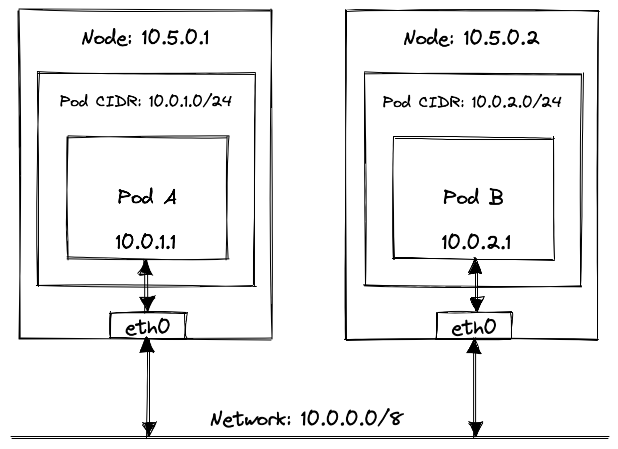
\includegraphics[width=\linewidth]{3-kube-networking.png}
    \caption{Connettività tra i \textit{Pod} in Kubernetes \cite{demystifying-kube-proxy}}
    \label{fig:kube_networking}
\end{figure}

È importante notare come alcuni plugin CNI fanno molto di più che garantire che i \textit{Pod} abbiano indirizzi IP e che possano parlare tra loro. Tuttavia per il nostro progetto è sufficiente considerare i plugin di CNI come la componente che assicura una connettività di livello 3 senza fare affidamento al NAT.

\subsection{Services}
A questo punto abbiamo capito come due \textit{Pod} comunicano usando i loro indirizzi IP. Tuttavia, a causa della natura effimera dei \textit{Pod}, non è quasi mai una buona idea usare direttamente gli indirizzi IP dei \textit{Pod} in quanto non sono persistenti tra i riavvii e possono cambiare senza preavviso, in risposta agli eventi che causano i riavvii (come fallimenti delle applicazioni, rollout, rollback, scale-up/down, ecc...).
Inoltre, quando si hanno più repliche di \textit{Pod} gestite da un oggetto padre, come un Deployment, tenere traccia di tutti gli indirizzi IP sul lato client potrebbe introdurre un overhead significativo. 

\begin{figure}[H]
    \centering
    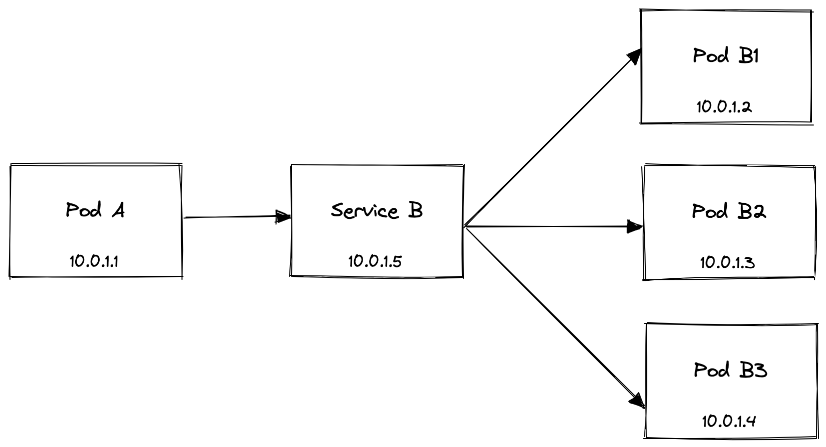
\includegraphics[width=\linewidth]{4-kubernetes-services.png}
    \caption{Schema dei \textit{Service}  in Kubernetes \cite{demystifying-kube-proxy}}
    \label{fig:kube_services}
\end{figure}

Per risolvere questo tipo di problematiche, sono stati introdotti i \textit{Service} che consentono di assegnare un singolo indirizzo IP virtuale a un insieme di Pod. Il servizio funziona tenendo traccia dello stato e degli indirizzi IP di un gruppo di \textit{Pod} e bilanciando il traffico verso di essi, come mostrato in \figurename~\ref{fig:kube_services}. In questo modo, il client può utilizzare l'indirizzo IP del servizio invece di affidarsi ai singoli indirizzi IP dei \textit{Pod} sottostanti.

\subsection{Endpoints}
Dobbiamo però capire come fanno i \textit{Service} a sapere quali \textit{Pod} esistono e sono pronti per accettare le richieste. Gli \textit{Endpoint} sono uno strumento che permette di adempiere a questo compito. 

Come illustrato in \figurename~\ref{fig:kube_endpoint} per ogni \textit{Service} esiste un Endpoint, che tiene traccia degli indirizzi IP dei \textit{Pod} che sono in esecuzione. È possibile pensare agli \textit{Endpoint} come a una tabella di ricerca per i Service, al fine di ottenere gli indirizzi IP dei \textit{Pod} di destinazione. 

\begin{figure}[H]
    \centering
    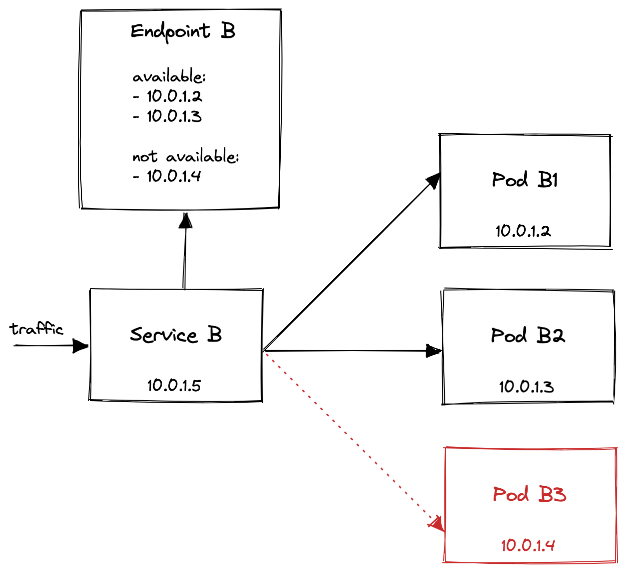
\includegraphics[width=\linewidth]{5-kubernetes-endpoint.png}
    \caption{Ruolo degli \textit{Endpoint}  in relazione ai \textit{Service}  in Kubernetes \cite{demystifying-kube-proxy}}
    \label{fig:kube_endpoint}
\end{figure}

È interessante notare come gli \textit{Endpoint}  non scalano bene con le dimensioni del cluster e il numero di \textit{Service} in esecuzione. A tal fine sono state introdotte le \textit{EndpointSlice}, che risolvono il problema della scalabilità.

\subsection{\texttt{iptables}}
\texttt{iptables} è un firewall per Linux estremamente utile, che permette di controllare i pacchetti a livello kernel. Per esempio, possiamo bloccare i pacchetti provenienti da un indirizzo IP specificato, o inoltrarli a un'interfaccia specifica, o ancora cambiare l'IP sorgente. Sono molte le attività che è possibile eseguire grazie a \texttt{iptables}.

È molto importante capire come funziona \texttt{iptables} per capire come funziona \texttt{kube-proxy} in quanto vedremo come quest'ultimo demandi le politiche di routing a \texttt{iptables} nella maggior parte dei casi.

\subsection{IPVS}
IPVS (IP Virtual Server) è un'evoluzione rispetto a \texttt{iptables}. Infatti quest'ultimo soffre di problemi di scalabilità: le regole sono valutate in modo sequenziale e nel caso di molti \textit{Pod} vengono create molte regole. Quindi nel caso si tratti di un'applicazione con molte richieste \texttt{iptables} tende a rallentare, come mostrato dal grafico in \figurename~\ref{fig:ipvs-vs-iptables}.

\begin{figure}[H]
    \centering
    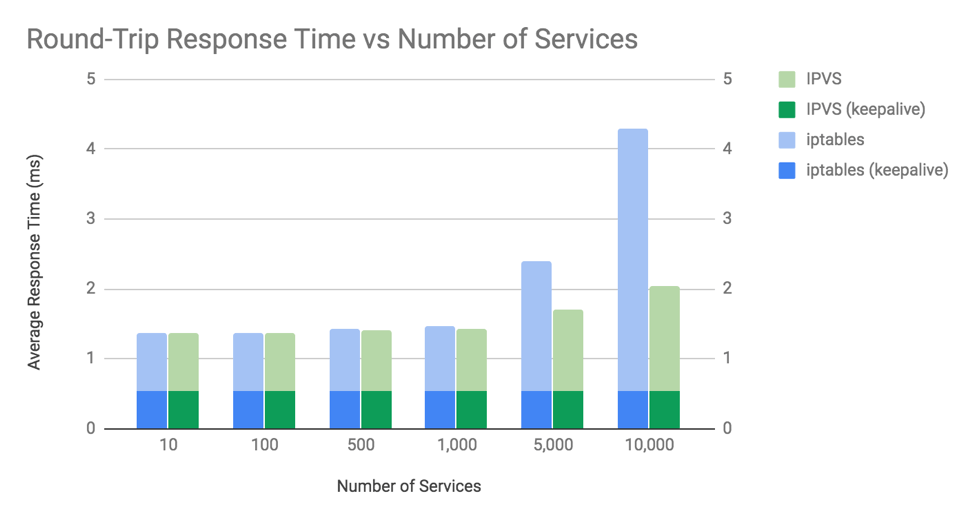
\includegraphics[width=\linewidth]{6-ipvs-vs-iptables.png}
    \caption{Comparazione delle performance di IPVS rispetto a \texttt{iptables} allo scalare del numero di \textit{Service} \cite{tigera-ipvs}}
    \label{fig:ipvs-vs-iptables}
\end{figure}

Lo useremo perché fornisce molte funzionalità di \textit{load balancing}, permettendo al traffico di essere inoltrato più efficacemente. Di seguito vediamo le politiche di scheduling proposte adottando IPVS:

\begin{itemize}
    \item round robin (\texttt{rr}) distribuisce le richieste equamente tra i nodi
    \item least connections (\texttt{lc}) assegna le richieste ai nodi col numero minore di richieste attive
    \item source hashing (\texttt{sh}) assegna le richieste ai nodi in base a una tabella di hash assegnata staticamente dall'indirizzo sorgente
    \item destination hashing (\texttt{dh}) assegna le richieste ai nodi in base a una tabella di hash assegnata staticamente dall'indirizzo di destinazione
    \item shortest expected delay (\texttt{sed}) assegna le richieste al nodo con la latenza attesa minore. La latenza è definita come 
    \begin{equation}
        \frac{(C_i + 1)}{U_i}
    \end{equation}
    rispetto al server \begin{math} i \end{math} dove \begin{math} C_i \end{math} è il numero di richieste attive e \begin{math} U_i \end{math} è un peso fissato per il server. 
    
    È importante quindi notare che questa metrica permette di selezionare il server col numero minore di richieste attive pesate per ogni server
    \item never queue (\texttt{nq}) assegna le richieste ai nodi senza richieste pendenti, senza aspettare che ce ne sia uno più veloce. Se tutti i server sono occupati viene adottata la politica \textit{shortest expected delay}
\end{itemize}

\subsection{\texttt{kube-proxy}}
Abbiamo detto che \texttt{kube-proxy} viene eseguito su ogni nodo di un cluster Kubernetes. Osserva gli oggetti \textit{Service} ed \textit{Endpoint} e di conseguenza aggiorna le regole di routing sui nodi per consentire la comunicazione tramite i \textit{Service}.

\texttt{kube-proxy} ha 4 modalità di esecuzione: \texttt{iptables}, IPVS, userspace e kernelspace. La modalità predefinita è \texttt{iptables}, dove le richieste vengono ripartite equamente tra i nodi, ma noi useremo IPVS per selezionare la politica di scheduling. È importante notare come \texttt{kube-proxy} non faccia distizione dal nodo a cui si fa richiesta.

Di seguito analizziamo più nel dettaglio la comunicazione tra \textit{Pod} e \textit{Service}.

\subsubsection{Pod to Service}
Quando viene creato il \textit{Service} la prima cosa che accade è che viene creato un corrispondente \textit{Endpoint} che memorizza la lista di \textit{Pod} a cui inoltrare le richieste. Quando l'\textit{Endpoint} è stato aggiornato con gli indirizzi IP corretti, tutti i \texttt{kube-proxy} dei nodi aggiornano le proprie regole di \texttt{iptables} con le nuove regole che impongono che i pacchetti al \textit{Service} vengano inoltrate ai nodi, selezionati in modo aleatorio.
Il processo di cambiare indirizzo IP di destinazione è chiamato anche \textit{Destination Network Address Translation} (DNAT) e possiamo osservarlo analizzando il processo illustrato in \figurename~\ref{fig:pod-to-service}.

\begin{figure}[H]
    \centering
    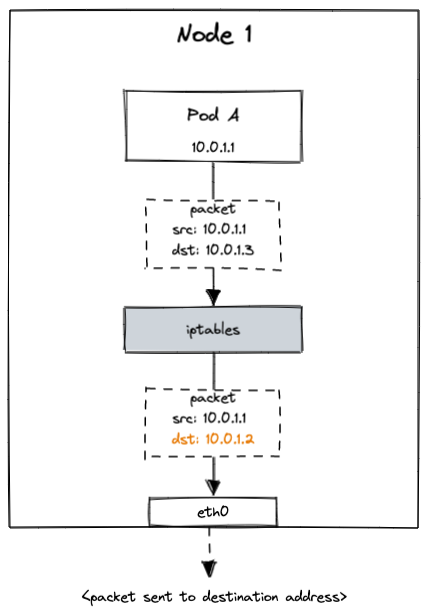
\includegraphics[width=8cm]{7-pod-to-service.png}
    \caption{Al pacchetto che proviene dal \textit{Pod A} viene cambiato IP di destinazione grazie a \texttt{iptables} \cite{demystifying-kube-proxy}}
    \label{fig:pod-to-service}
\end{figure}

\subsubsection{Service to Pod}
Oltre al funzionamento intuitivo della comunicazione inversa è necessario istruire \texttt{iptables} per cambiare IP sorgente dei pacchetti che giungono come risposta a una comunicazione in cui sono state sfruttate le funzionalità DNAT. Questo è possibile grazie alla funzione \textit{conntrack} che permette di ricordare le scelte di routing intraprese in precedenza con un processo che viene chiamato \textit{Source NAT} (SNAT), illustrato in \figurename~\ref{fig:service-to-pod}.

\begin{figure}[H]
    \centering
    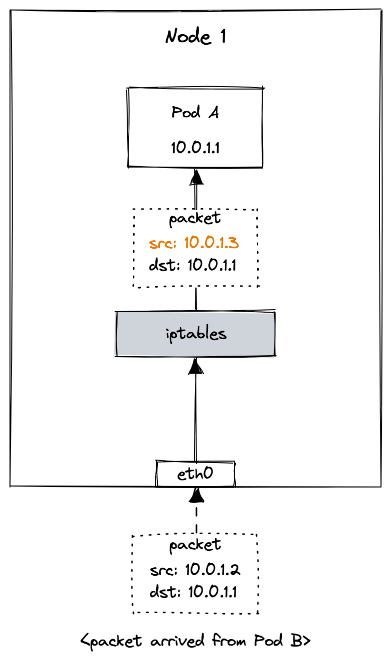
\includegraphics[width=8cm]{8-service-to-pod.png}
    \caption{Al pacchetto che proviene dal \textit{Pod B} viene cambiato IP sorgente grazie a \texttt{iptables} \cite{demystifying-kube-proxy}}
    \label{fig:service-to-pod}
\end{figure}

\addcontentsline{toc}{chapter}{Progettazione}  
\chapter{Progettazione}

In questo capitolo tratteremo la progettazione dell'ambiente di emulazione, ponendo particolare attenzione all'architettura di rete. Successivamente, analizzeremo le possibili anomalie che si possono presentare e mostreremo la reazione del sistema.

\section{Componenti e connessioni}
\subsection{Scopo del progetto}
Per ideare correttamente l'ambiente di emulazione dobbiamo mettere correttamente a fuoco l'obiettivo del progetto. Vogliamo progettare un ambiente di emulazione per comprendere il funzionamento e le prestazioni delle tecnologie di \textit{edge computing}. Inoltre è importante porre particolare attenzione alla compatibilità dell'ambiente con la struttura della rete cellulare di quinta generazione (5G) per estendere lo studio a quest'ultima.

Vedremo di seguito quali scelte progettuali abbiamo intrapreso per rispondere meglio alle esigenze del sistema di emulazione. 

\subsection{Requisiti}
Per comprendere le scelte di progettazione dobbiamo evidenziare i requisiti che l'ambiente di emulazione dovrà soddisfare.

\begin{itemize}
    \item Compatibilità con le tecnologie di edge computing e reti mobili 5G: dato l'obiettivo del progetto è fondamentale che l'ambiente di emulazione consenta lo studio e l'analisi di queste tecnologie.

    \item Componenti e connessioni: L'ambiente di emulazione deve essere composto da più di un punto di accesso e da più di una macchina in grado di eseguire l'applicazione.

    \item Latenza arbitraria: I collegamenti tra le antenne e i nodi devono presentare una latenza arbitraria basata sulla distanza geografica che si desidera simulare. Questo permette di valutare l'impatto della latenza sulla distribuzione delle richieste e sulle prestazioni complessive del sistema.

    \item Competitività dei nodi: Il sistema deve essere in grado di determinare la competitività dei nodi in base al tempo di risposta alle richieste. La scelta del nodo più competitivo avviene considerando sia il delay sul link tra le antenne e i nodi, sia il tempo di elaborazione dei nodi stessi.
\end{itemize}

\subsection{Schema generale}
L'ambiente di emulazione deve essere composto da più di un punto di accesso e da più di una macchina in grado di eseguire l'applicazione. Abbiamo scelto di mantenere una progettazione snella, favorendone la semplicità e l'efficacia, considerando due antenne 5G connesse a entrambe le macchine.

Ogni macchina sarà un nodo di un cluster di un sistema di orchestrazione. Abbiamo deciso di adottare questa soluzione in quanto è quella che risponde maggiormente alle nostre necessità.

Come viene mostrato in \figurename~\ref{fig:schema-generale}, il nodo \textit{control plane} non è direttamente collegato alle antenne, che invece sono collegate a entrambi i nodi. I collegamenti tra le antenne e i nodi subiscono una latenza arbitraria basata sulla distanza geografica che vogliamo simulare.

\begin{figure}[h]
    \centering
    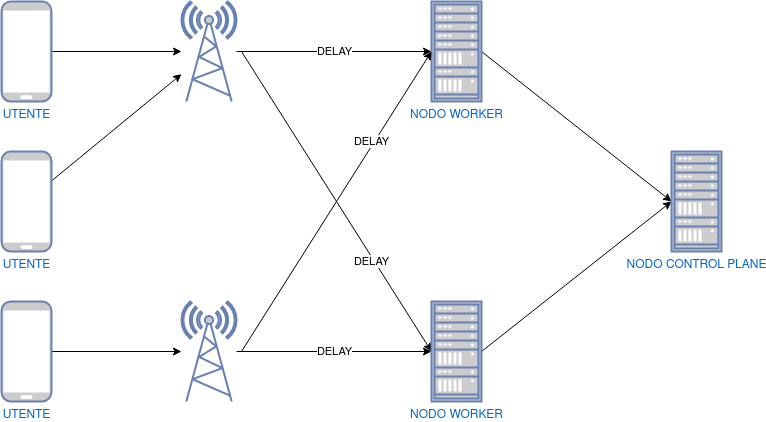
\includegraphics[width=\linewidth]{9_schema_generale.png}
    \caption{Schema generale dell'architettura proposta}
    \label{fig:schema-generale}
\end{figure}

\section{Schema di funzionamento}

\subsection{Funzionamento ideale}
Avendo chiaro lo schema dei componenti e delle relative connessioni possiamo descrivere il funzionamento dell'architettura costruita in una situazione senza anomalie.

L'utente richiede l'applicazione, la quale è stata precedentemente \textit{istanziata} su tutti i nodi worker che rende possibile fare richiesta ad entrambi i nodi per ottenere una risposta alla richiesta. La richiesta viene inoltrata al nodo più \textit{competitivo}. 

Il concetto di competitività lo associamo al nodo che riesce a rispondere alla richiesta nel minor tempo possibile. Questo tempo tiene in considerazione sia il delay sul link tra le antenne e i nodi, sia il tempo di elaborazione dei nodi. Entrambe queste metriche non potranno che essere stimate.

\subsection{Aumento del numero di utenti}
\subsubsection{Globalmente}
Analizziamo ora il caso di un aumento improvviso degli utenti che si servono dell'applicazione. Possiamo distinguere due casi: quello in cui gli utenti aumentano globalmente in modo uniforme o quella in cui aumentano in una regione geografica definita. Procediamo ad analizzare il primo caso.

Dato l'aumento delle richieste viene aumentato il numero di \textit{Pod} presenti sui nodi worker, proporzionalmente alla capacità computazionale e al carico. Questo permette di far fronte alle richieste finché le risorse hardware non esauriscono.

\subsubsection{In una sola area geografica}
Più particolare è il caso di un aumento sproporzionato di utenti in una sola area geografica. Questo evento porta il numero di richieste ad aumentare sensibilmente sui nodi di quell'area geografica, e in modo minore su tutti gli altri nodi. Le richieste aumentano in modo inversamente proporzionale rispetto alla latenza tra il punto di accesso e il nodo.

In questo caso il numero di \textit{Pod} viene aumentato in modo proporzionale all'aumento delle richieste. In caso di esaurimento delle risorse hardware le richieste vengono dirottate verso nodi più distanti ma in grado di rispondere complessivamente prima alle richieste. Questo in virtù del concetto di competitività a cui abbiamo accennato in precedenza.

\section{Possibili anomalie}

\subsection{Fallimento di un nodo}
Vediamo ora le possibili anomalie che si potrebbero presentare nell'architettura della rete. Una prima eventualità che vogliamo considerare è quella del fallimento di un nodo. Intendiamo, quindi, tutti quei casi in cui un nodo non possa più adempiere alle richieste degli utenti, in seguito a problemi hardware, software o dell'interruzione della connettività di rete. 

In questi casi le richieste che sarebbero state inoltrate al nodo in questione vengono ripartite agli altri nodi, che si fanno carico delle richieste in proporzione al delay tra gli utenti. Assumendo che il delay sia proporzionale alla distanza geografica tra i nodi, le richieste verranno inoltrare ai nodi più vicini geograficamente, come illustrato in \figurename~\ref{fig:anomalia-fallimento-di-un-nodo}.

\begin{figure}[H]
    \centering
    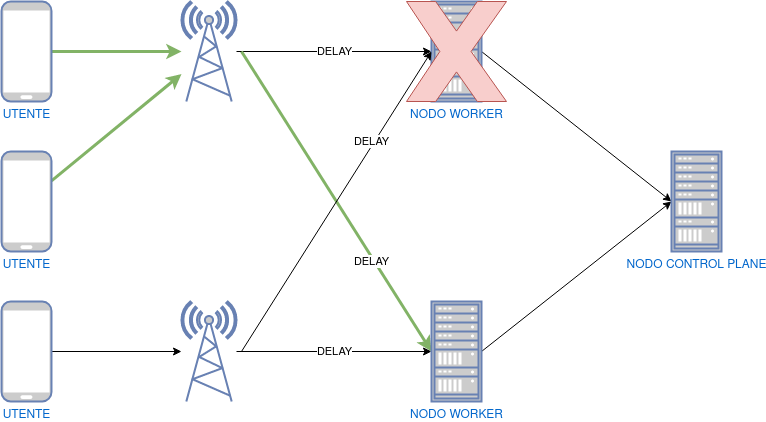
\includegraphics[width=\linewidth]{10_anomalia-fallimento-di-un-nodo.png}
    \caption{Schema generale dell'architettura in cui un nodo non è più disponibile. In questo caso le richieste vengono inoltrate ai nodi più competenti.}
    \label{fig:anomalia-fallimento-di-un-nodo}
\end{figure}

\subsection{Fallimento del nodo \textit{control plane}}
Una seconda eventualità che potrebbe accadere è il fallimento del nodo \textit{control plane}. Questo porta il cluster a non funzionare più correttamente, portando il comportamento a non essere più deterministico. Come mostriamo in \figurename~\ref{fig:anomalia-fallimento-control-plane}, è ragionevole assumere che le richieste non vengano più soddisfatte in tutto il cluster. È quindi importante porre l'accento sull'\textit{high availability} del nodo \textit{control plane}, principalmente tramite la replicazione hardware che consente di adottare la metodologia chiamata \textit{hot swap}.

Nella nostra architettura non saranno presenti queste accortezze in quanto la disponibilità non è un fattore chiave nella buona riuscita del progetto. L'argomento può essere approfondito con la necessaria dovizia di particolari, tuttavia lo abbiamo solo accennato per evidenziare quello che è un \textit{single point of failure} nell'architettura.

\begin{figure}[H]
    \centering
    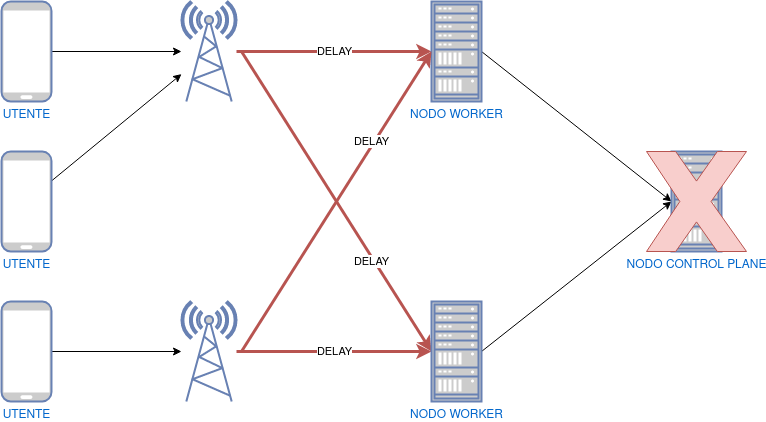
\includegraphics[width=\linewidth]{11_anomalia-fallimento-control-plane.png}
    \caption{Schema generale dell'architettura in cui il nodo \textit{control plane} non è più disponibile. Il cluster smette di funzionare.}
    \label{fig:anomalia-fallimento-control-plane}
\end{figure}

\subsection{Delay incrementato}
Prendiamo in considerazione un'eventualità che non interrompe il servizio ma ne modifica il comportamento. Nel caso il delay tra un punto di accesso e un nodo aumenti notevolmente le richieste non verranno più distribuite equamente, in quanto la competitività diventa minore per il nodo collegato al link col delay aumentato. Come è possibile notare in \figurename~\ref{fig:anomalia-aumento-delay}, questo porterà la rete a ribilanciarsi: i nodi vicini diventeranno più competitivi all'aumentare del delay sul nodo. 

\begin{figure}[H]
    \centering
    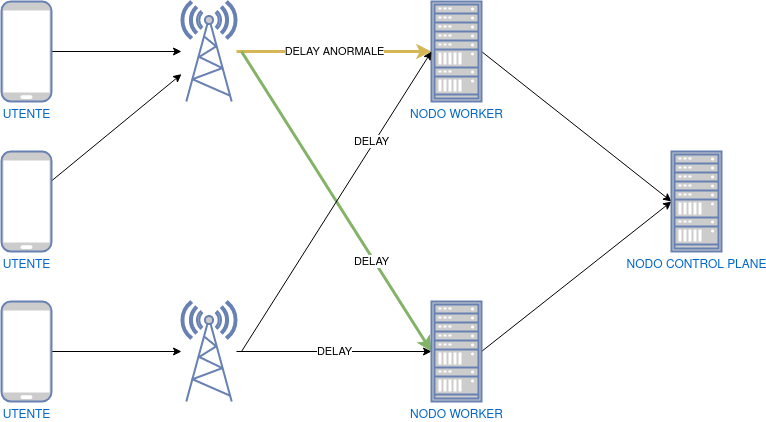
\includegraphics[width=\linewidth]{12_anomalia-aumento-delay.png}
    \caption{Schema generale dell'architettura in cui il link tra un nodo e un punto di accesso ha un delay incrementato. Il cluster si ribilancia e le richieste vengono inoltrate ai nodi più competitivi.}
    \label{fig:anomalia-aumento-delay}
\end{figure}

\addcontentsline{toc}{chapter}{Implementazione}  
\chapter{Implementazione}

%\section{Introduzione}
In questo capitolo mostreremo i dettagli implementativi della struttura del progetto. Descriveremo i componenti hardware e software più significativi capiremo le modifiche apportate alla parte di networking del progetto.

\section{Struttura del \textit{testbed}}

\subsection{Hardware}
Adottiamo un approccio \textit{bottom-up} per la descrizione dell'implementazione adottata per il progetto, partendo dalle componenti hardware. 

Nonostante vogliamo implementare un cluster di orchestrazione con più nodi abbiamo scelto di usare un singolo server. Quest'ultimo è dotato di una singola interfaccia di rete fisica. Vedremo di seguito le tecnologie che abbiamo sfruttato per la creazione dei nodi.

\subsection{Virtualizzazione}
Per creare più nodi abbiamo scelto di creare più macchine virtuali sulla singola macchina fisica, varando diversi \textit{hypervisor}. Nonostante la popolarità delle tecnologie VMWare, e in particolare di VMWare vSphere in ambito cloud, abbiamo deciso di adottare il sistema Proxmox Virtual Environment (PVE), di cui mostriamo la schermata di gestione in \figurename~\ref{fig:schermata-proxmox}. 

Quest'ultimo è un \textit{hypervisor} open source che sfrutta la funzionalità \texttt{KVM} del kernel Linux per la virtualizzazione. Di seguito elenchiamo i motivi che hanno portato alla nostra scelta:

\begin{itemize}
    \item il sistema di Proxmox è open source e non è altro che un sistema operativo Linux basato sulla distribuzione Debian. Queste caratteristiche permettono di studiarne a fondo il comportamento ed eventualmente di modificarlo
    \item è un software gratuito nella versione \textit{Community Edition}
    \item il supporto della community è ampio così come la documentazione
\end{itemize}

\begin{sidewaysfigure}[ht]
    \centering
    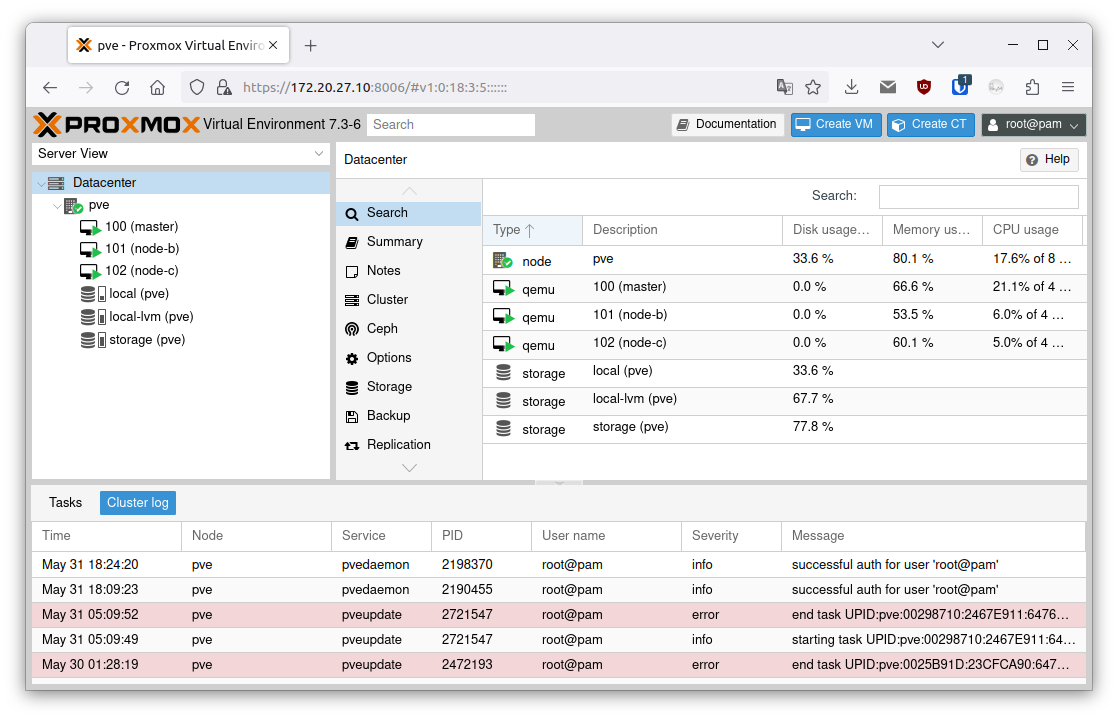
\includegraphics[width=\linewidth]{13_schemata-proxmox.png}
    \caption{Schermata principale di Proxmox Virtual Environment con le tre macchine virtuali configurate e attive}
    \label{fig:schermata-proxmox}
\end{sidewaysfigure}

Abbiamo scelto di usare Ubuntu Server 22.04 come sistema operativo per le macchine virtuali.

\subsection{Sistema di orchestrazione}
Come è stato anticipato più volte abbiamo scelto di usare Kubernetes (K8s) come sistema di orchestrazione in quanto è la principale tecnologia disponibile ed è lo standard \textit{de facto} in ambito cloud. 

Come mostrato in \figurename~\ref{fig:schema-implementazione}, ogni macchina virtuale è un nodo di Kubernetes, ognuna con le stesse risorse hardware allocate. Abbiamo installato \texttt{containerd} come \textit{container runtime} e \texttt{kubeadm} su tutti i nodi e \texttt{kubectl} sul nodo \textit{control plane}.
Infine abbiamo inizializzato il nodo \textit{control plane}.
\begin{lstlisting}[language=bash]
  $ sudo kubeadm init
\end{lstlisting}

\begin{figure}[H]
    \centering
    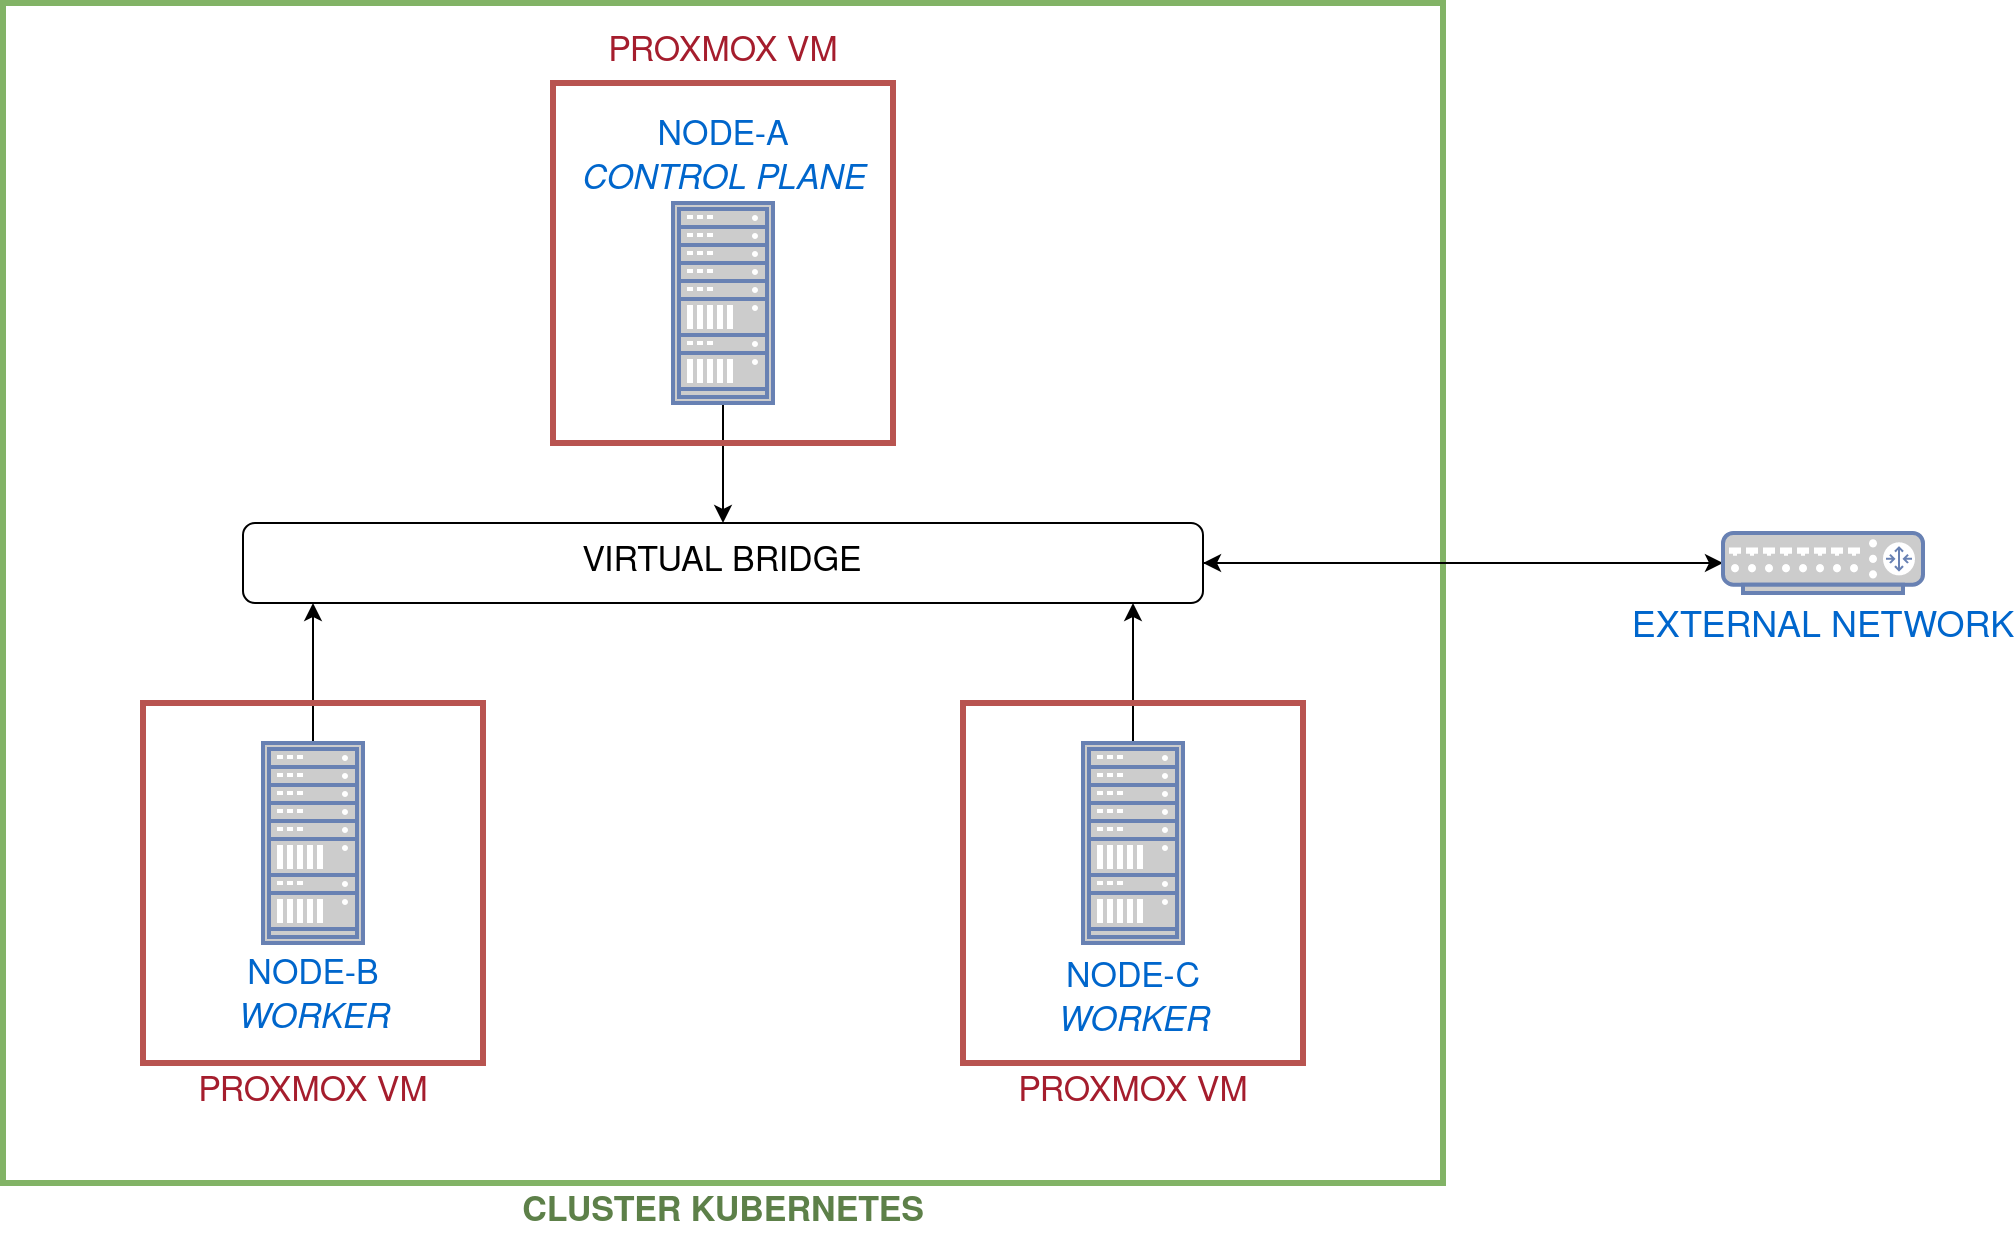
\includegraphics[width=\linewidth]{16_schema-implementazione.png}
    \caption{Schema generale dell'implementazione dell'architettura}
    \label{fig:schema-implementazione}
\end{figure}

\subsection{Networking}
\subsubsection{Kubernetes networking}
Come abbiamo scritto in precedenza il networking tra i nodi in Kubernetes è gestito da dei plugin appositi. Abbiamo scelto di adottare il plugin Calico per questa funzione, la cui installazione è possibile tramite un file di configurazione di Kubernetes in formato YAML, come tutte le altre configurazioni che andremo a creare.

\subsubsection{VM networking}
Abbiamo scelto di esporre la macchina fisica con un indirizzo IP, appartenente alla sottorete del laboratorio, e di creare una rete interna per le macchine virtuali. Questo permetterà di gestire più facilmente le configurazioni alle interfacce che andremo a creare. 

Per raggiungere questo risultato abbiamo modificato la configurazione del sistema operativo. La facilità di configurazione delle interfacce è dovuta alla scelta di Proxmox come hypervisor. Di seguito riportiamo il file \texttt{/etc/network/interfaces} modificato in cui possiamo notare come siano state inserite delle regole statiche di routing per poter accedere ai nodi dall'indirizzo IP della macchina fisica.

\begin{lstlisting}
auto lo
iface lo inet loopback

auto enp3s0
iface enp3s0 inet static
        address  172.20.27.10/28
        gateway  172.20.27.1

auto vmbr0
iface vmbr0 inet static
        address  192.168.0.1/24
        bridge-ports none
        bridge-stp off
        bridge-fd 0
        
post-up   echo 1 > /proc/sys/net/ipv4/ip_forward
post-up   iptables -t nat -A POSTROUTING -s '192.168.0.0/24' -o enp3s0 -j MASQUERADE
post-up   iptables -t nat -A PREROUTING -i enp3s0 -p tcp -m tcp --dport 10022 -j DNAT --to-destination 192.168.0.100:22
post-up   iptables -t nat -A PREROUTING -i enp3s0 -p tcp -m tcp --dport 10122 -j DNAT --to-destination 192.168.0.101:22
post-up   iptables -t nat -A PREROUTING -i enp3s0 -p tcp -m tcp --dport 10222 -j DNAT --to-destination 192.168.0.102:22
post-up   iptables -t nat -A PREROUTING -i enp3s0 -p tcp -m tcp --dport 30000 -j DNAT --to-destination 192.168.0.100:30000
post-up   iptables -t nat -A PREROUTING -i enp3s0 -p tcp -m tcp --dport 30001 -j DNAT --to-destination 192.168.0.101:30000
post-up   iptables -t nat -A PREROUTING -i enp3s0 -p tcp -m tcp --dport 30002 -j DNAT --to-destination 192.168.0.102:30000
post-down iptables -t nat -D POSTROUTING -s '192.168.0.0/24' -o enp3s0 -j MASQUERADE
\end{lstlisting}

\subsection{\texttt{kube-proxy}}
È possibile modificare la configurazione di \texttt{kube-proxy} modificando la \textit{ConfigMap} associata al componente. Per farlo usiamo il comando appropriato di \texttt{kubectl}:
\begin{lstlisting}[language=bash]
  $ kubectl edit configmap kube-proxy -n kube-system
\end{lstlisting}

Nel nostro caso vogliamo modificare la modalità da \texttt{iptables} a IPVS. Sempre nella stessa schermata di configurazione cambieremo anche l'algoritmo di scheduling. 

\section{Network degradation}

\subsection{Ritardi sulle interfacce}
Vogliamo creare un ritardo artificiale sulle interfacce. Ogni VM su Proxmox è connessa alla rete tramite un'interfaccia di rete dedicata, grazie a cui possiamo applicare un ritardo specifico per ogni macchina virtuale. Per farlo sfruttiamo il famoso tool \texttt{tc-netem}.

Poniamo il nome dell'interfaccia come \texttt{tap100i0}, che identifica l'interfaccia 0 della macchina virtuale con ID 100 e aggiungiamo un ritardo di 1000 ms ai pacchetti in uscita col seguente comando.

\begin{lstlisting}[language=bash]
  $ tc qdisc add dev tap100i0 root netem delay 1000ms
\end{lstlisting}

Per rimuovere il ritardo usiamo invece il comando

\begin{lstlisting}[language=bash]
  $ tc qdisc del dev tap100i0 root netem
\end{lstlisting}

\subsubsection{Ritardo iterativo incrementale}
Questi comandi possono essere inseriti in uno script che permette di aumentare iterativamente i ritardi su un'interfaccia che permette di testare la risposta dello scheduling al variare della latenza.

Nel codice riportato di seguito incrementiamo la latenza da 1ms a 4096ms, raddoppiandola ogni volta. Questa operazione viene svolta ogni 15 secondi sull'interfaccia specificata.

\begin{lstlisting}[language=bash]
#!/bin/bash

X=1

while [ $X -le 4096 ]
do
    tc qdisc del dev tap101i0 root netem ; tc qdisc add dev tap101i0 root netem delay ${X}ms rate 1mbit
    echo "Delay impostato a ${X}ms. Attendo 15 secondi..."
    sleep 15
    X=$((X*2))
done
tc qdisc del dev tap101i0 root netem
\end{lstlisting}

\subsection{Limite al throughput}
Per i pacchetti in ingresso possiamo anche restringere le potenzialità di trasferimento della rete. Vediamo un esempio di comandi per portare la banda a 1mbps, sempre sull'interfaccia  \texttt{tap100i0}.

\begin{lstlisting}[language=bash]
  $ tc qdisc add dev tap100i0 ingress
  $ tc filter add dev tap100i0 parent ffff: protocol ip prio 1 u32 match ip src 0.0.0.0/0 police rate 1mbit burst 10k drop flowid :1
\end{lstlisting}

Anche in questo caso mostriamo anche i comandi per rimuovere il ritardo.

\begin{lstlisting}[language=bash]
  $ tc filter del dev tap100i0 parent ffff: protocol ip prio 1 u32
  $ tc qdisc del dev tap100i0 ingress
\end{lstlisting}

\subsection{Ritardi selettivi}
Grazie all'implementazione adottata le macchine virtuali comunicano all'esterno della loro rete locale tramite l'indirizzo della macchina fisica. Tuttavia, vogliamo essere in grado di applicare dei ritardi più granulari, in base alla sorgente dei pacchetti. Questa accortezza ci permette di simulare i ritardi tra nodi e punti di accesso diversi avendo una sola interfaccia. Dati gli indirizzi IP dei punti di accesso, possiamo applicare un ritardo specifico per ogni link virtuale, avendo un solo link fisico. 

Dopo averne elencato i vantaggi vediamo come applicare un ritardo selettivo sull'interfaccia \texttt{tap100i0} per i pacchetti provenienti dall'indirizzo IP \texttt{192.168.1.1}.

\begin{lstlisting}[language=bash]
  $ tc qdisc add dev tap100i0 root handle 1: prio
  $ tc filter add dev tap100i0 protocol ip parent 1: prio 1 u32 match ip src 192.168.1.1 flowid 1:1
  $ tc qdisc add dev tap100i0 parent 1:1 netem delay 100ms
\end{lstlisting}

Come in precedenza forniamo anche il comando per rimuovere la regola.

\begin{lstlisting}[language=bash]
  $ tc qdisc del dev tap100i0 root handle 1: prio
\end{lstlisting}

\section{Simulatore}
\subsection{Server}
Per poter verificare il comportamento del cluster e apprezzare i cambiamenti allo scheduling sui nodi abbiamo creato un'applicazione di test in Python che sfrutta la libreria \texttt{flask} per la creazione di un endpoint di un'API. 

Ricevuta una richiesta, il server attenderà un tempo casuale prima di rispondere che viene estratto da una distribuzione esponenziale con parametri forniti. IL tempo viene indicato nella risposta inviata al client.

L'applicazione sfrutta i thread per poter gestire più richieste contemporaneamente e durante il tempo di attesa lo script, grazie al tool da linea di comando \texttt{stress-ng}, occuperà la CPU per una percentuale data.

\begin{lstlisting}[language=Python]
from flask import Flask
import random
import time
import subprocess
import threading
import multiprocessing
import os

app = Flask(__name__)

# tempo medio di risposta in secondi
tempo_medio = os.getenv('FLUFFY_AVG_TIME', 20)

# percentuale di CPU da occupare in caso di richieste in fase di elaborazione
percentuale_cpu = os.getenv('FLUFFY_CPU_PERCENT', 80)

def occupa_cpu():
    # avvia stress-ng per occupare la CPU
    subprocess.run(["stress-ng", "--cpu", str(multiprocessing.cpu_count()), "--cpu-load", str(percentuale_cpu)])

@app.route('/')
def api():
    # genera un tempo di attesa casuale
    tempo_attesa = random.expovariate(1/tempo_medio)
    
    # avvia il thread per occupare la CPU
    t = threading.Thread(target=occupa_cpu)
    t.start()

    # metti in pausa il processo per il tempo di attesa casuale
    time.sleep(tempo_attesa)

    # ferma lo stress-ng
    subprocess.run(["pkill", "stress-ng"])

    return 'Risposta dopo {:.2f} secondi'.format(tempo_attesa)

if __name__ == '__main__':
    print(f"Cores: {multiprocessing.cpu_count()}")
    print(f"Avg time: {tempo_medio}")
    print(f"Percent CPU: {percentuale_cpu}")
    app.run(host='0.0.0.0', port=5000)
\end{lstlisting}

\subsection{Container}
Dopo aver creato il file \texttt{requirements.txt} dobbiamo create il Dockerfile per poter costruire un container da poter \textit{deployare} nel cluster. Nel Dockerfile dovremo indicare di installare anche il pacchetto \texttt{stress-ng}.

\begin{lstlisting}
# Usa un'immagine di Python come base
FROM python:3.9-slim
RUN /bin/sh -c set -eux; apt-get update; apt-get install -y --no-install-recommends stress-ng procps 

# Copia il codice sorgente nella directory /app del container
COPY . /app

# Imposta la directory di lavoro come /app
WORKDIR /app

# Installa le dipendenze del codice sorgente
RUN pip install -r requirements.txt

# Espone la porta 8000 del container
EXPOSE 5000

# Avvia il server quando il container viene avviato
CMD [ "python", "server.py" ]
\end{lstlisting}

\subsection{Kubernetes \textit{Deployment}}
Per eseguire l'applicazione server sui nodi dobbiamo creare un \textit{Deployment} di Kubernetes in formato YAML. Questo file fornirà le informazioni necessarie a Kubernetes per l'esecuzione, compresi il nome del container di riferimento e il numero di \textit{Pod} da istanziare. 

Nello stesso file abbiamo specificato il \textit{Service} associato, che permette di accedere all'applicazione. Per applicare la configurazione possiamo usare il comando \texttt{kubectl apply}.

\begin{lstlisting}
apiVersion: apps/v1
kind: Deployment
metadata:
  name: simulator
spec:
  replicas: 4
  selector:
    matchLabels:
      app: simulator
  template:
    metadata:
      labels:
        app: simulator
    spec:
      containers:
      - name: simulator-server
        image: mrriky54/fluffy-simulator
        ports:
        - containerPort: 5000
---
apiVersion: v1
kind: Service
metadata:
  name: simulator-service
spec:
  selector:
    app: simulator
  ports:
    - protocol: TCP
      port: 5000
      targetPort: 5000
      nodePort: 30000
  type: NodePort
\end{lstlisting}

\subsection{Client}
Ora poniamo l'attenzione sullo script per creare le richieste, anch'esso scritto in linguaggio Python. Iniziamo importando le librerie necessarie e allocando le variabili globali.

\begin{lstlisting}[language=Python]
import requests
import random
import time
from bs4 import BeautifulSoup
import threading

SERVER = "172.20.27.10"  # Sostituisci con il tuo server
PORT = 30000  # Sostituisci con la tua porta
MEAN_INTERVAL = 60  # Sostituisci con la media dell'intervallo di tempo tra una richiesta e l'altra
\end{lstlisting}

Definiamo poi la funzione per l'invio di una richiesta, che permette di tenere traccia del tempo trascorso e di gestire gli eventuali errori.

\begin{lstlisting}[language=Python]
def send_request():
    url = "http://{}:{}/".format(SERVER, PORT)
    start_time = time.time()
    try:
        response = requests.get(url, timeout=120)
    except requests.exceptions.Timeout:
        print(f"Timeout scaduto per la richiesta")
    else:
        if response.status_code != 200:
            print("Errore durante la richiesta HTTP")
        else:
            elapsed_time = time.time() - start_time
            print(f"{response.content}")
\end{lstlisting}

Il \textit{main} dell'applicazione non farà altro che inviare più richieste, attendendo un tempo casuale estratto da una distribuzione esponenziale. Il programma non termina.

\begin{lstlisting}[language=Python]
while True:
    
    # Invia la richiesta HTTP in un thread separato
    print("Invio una richiesta")
    t = threading.Thread(target=send_request, args=())
    t.start()

    # Calcola il prossimo intervallo di tempo
    next_interval = random.expovariate(1/MEAN_INTERVAL)

    # Attendi per il prossimo intervallo di tempo o per la fine delle richieste in corso
    print(f"Attendo {next_interval:.2f} secondi")
    time.sleep(next_interval)
\end{lstlisting}

\addcontentsline{toc}{chapter}{Analisi dei risultati}  
\chapter{Analisi dei risultati}

%\section{Introduzione}
In questo capitolo analizzeremo i dati ottenuti dal nostro \textit{testbed}. Nello specifico, descriveremo come abbiamo raccolto i dati e quali abbiamo ritenuto essere le informazioni più significative relativamente al funzionamento del sistema.

Successivamente rappresenteremo i dati in forma grafica per comprendere le caratteristiche degli algoritmi di scheduling, limitatamente alla struttura del nostro progetto.

\section{Raccolta dei dati}
\subsection{Configurazione della struttura}
Per ottenere in modo completo tutti i dati necessari all'analisi dobbiamo considerare la struttura del progetto. Come possiamo notare in \figurename~\ref{fig:schema-generale_res}, abbiamo due nodi worker che risponderanno alle richieste, che saranno presenti anche per quanto riguarda la raccolta dei dati.

I due nodi avranno una distanza geografica simulata, ovvero un ritardo artificiale sul link che li collega agli endpoint. Nello specifico consideriamo un ritardo di 50 millisecondi per il \texttt{node B} e un ritardo di 5 millisecondi per il \texttt{node C}.

\begin{figure}[h]
    \centering
    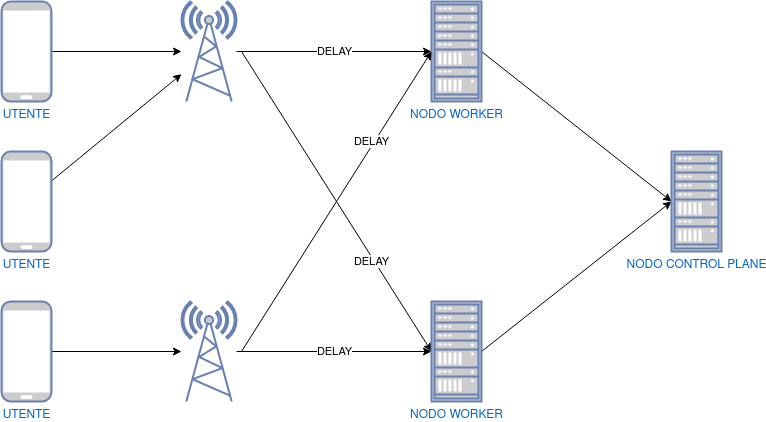
\includegraphics[width=\linewidth]{9_schema_generale.png}
    \caption{Schema generale dell'architettura proposta}
    \label{fig:schema-generale_res}
\end{figure}

\subsection{Scenari}
Consideriamo diversi scenari in cui l'applicazione può trovarsi, che corrispondono a diverse configurazioni di carico. Vogliamo quindi aumentare il numero medio di richieste per secondo e controllare come reagisce l'inoltro delle richieste.

Per simulare le richieste e il ritardo tra queste scegliamo di attendere un tempo aleatorio, estratto da una distribuzione esponenziale con parametri fissati al fine di ottenere in media il numero di richieste al secondo che desideriamo.

Questa operazione la decliniamo per i vari scheduler che vogliamo considerare: Round-Robin (\texttt{rr}), Least Connections (\texttt{lc}) e Shortest Expected Delay (\texttt{sed}). Abbiamo descritto questi scheduler nei capitoli precedenti, evidenziando le loro differenze e peculiarità. Per permetterci di selezionare questi scheduler dobbiamo usare \texttt{IPVS} come tecnologia sottostante per l'inoltro delle richieste.

\subsection{Le \textit{run}}
Per ogni scenario vogliamo ottenere un numero congruo di dati. A tal fine genereremo 5000 richieste per ogni scenario, divise in 100 richieste per 50 seed della libreria random. Grazie a questa configurazione riusciamo a raccogliere un numero congruo di dati mantenendo la replicabilità.

\subsection{Valori raccolti}
Per ogni richiesta raccogliamo alcune informazioni riguardo la gestione della richiesta stessa.

\begin{itemize}
    \item \texttt{node}: il nodo a cui è stata inoltrata la richiesta
    \item \texttt{delay}: il delay applicato al link che collega il nodo agli altri, misurato in millisecondi.
    \item \texttt{simulated\_time}: il valore (in secondi) che viene simulato lato server per la gestione della richiesta. È estratto dalla distribuzione esponenziale con media pari a 100 millisecondi.
    \item \texttt{actual\_time}: il tempo (in secondi) misurato lato client per la ricezione della risposta. Considerare come cambia questo valore in funzione del \texttt{simulated\_time} ci permette di parlare della bontà di uno scheduler.
\end{itemize}

\begin{table}[H]
\begin{center}
\begin{tabular}{ |m{13em}|m{20em}| } 
 \hline
 \texttt{scheduler} & È il tipo di scheduler usato. Può essere Round-Robin, Least Connections o Shortest Expected Delay. \\
 \hline
 \texttt{time\_between\_requests} & Corrisponde al tempo medio tra le richieste \\
 \hline
 \texttt{seed} & È il seed usato per la \textit{run} \\
 \hline
 \texttt{index} & Corrisponde all'indice della richiesta, univoco all'interno di una stesso scenario e seed \\
 \hline
 \texttt{node} & È il nodo a cui lo scheduler ha inoltrato la richiesta \\
 \hline
 \texttt{delay} & Corrisponde al delay introdotto sul link che collega il nodo, in millisecondi \\
 \hline
 \texttt{simulated\_time} & È il tempo di computazione simulato lato server per la richiesta, in secondi \\
 \hline
 \texttt{actual\_time} & Consiste nel tempo misurato lato client per ottenere la risposta alla richiesta, in secondi \\
 \hline
\end{tabular}
\end{center}
\caption{Tabella riassuntiva dei valori raccolti}
\label{table:1}
\end{table}

\section{Analisi del RTT}

Vogliamo confrontare le performance dei vari scheduler all'aumentare del numero di richieste, per capire in quale scenario è più appropriato ciascun algoritmo. Per farlo useremo il round trip time (RTT) medio per rispondere ad una richiesta, misurato lato client, che ci consentirà di parlare delle performance degli algoritmi nella nostra architettura. 
Analizzando il RTT al variare del numero di richieste al secondo capiremo quanto gli algoritmi di scheduling analizzati siano resilienti all'aumentare del carico e quali, invece, siano più adatti a situazioni in cui le risorse hardware sono mediamente sovradimensionate. 

\begin{figure}[H]
    \centering
    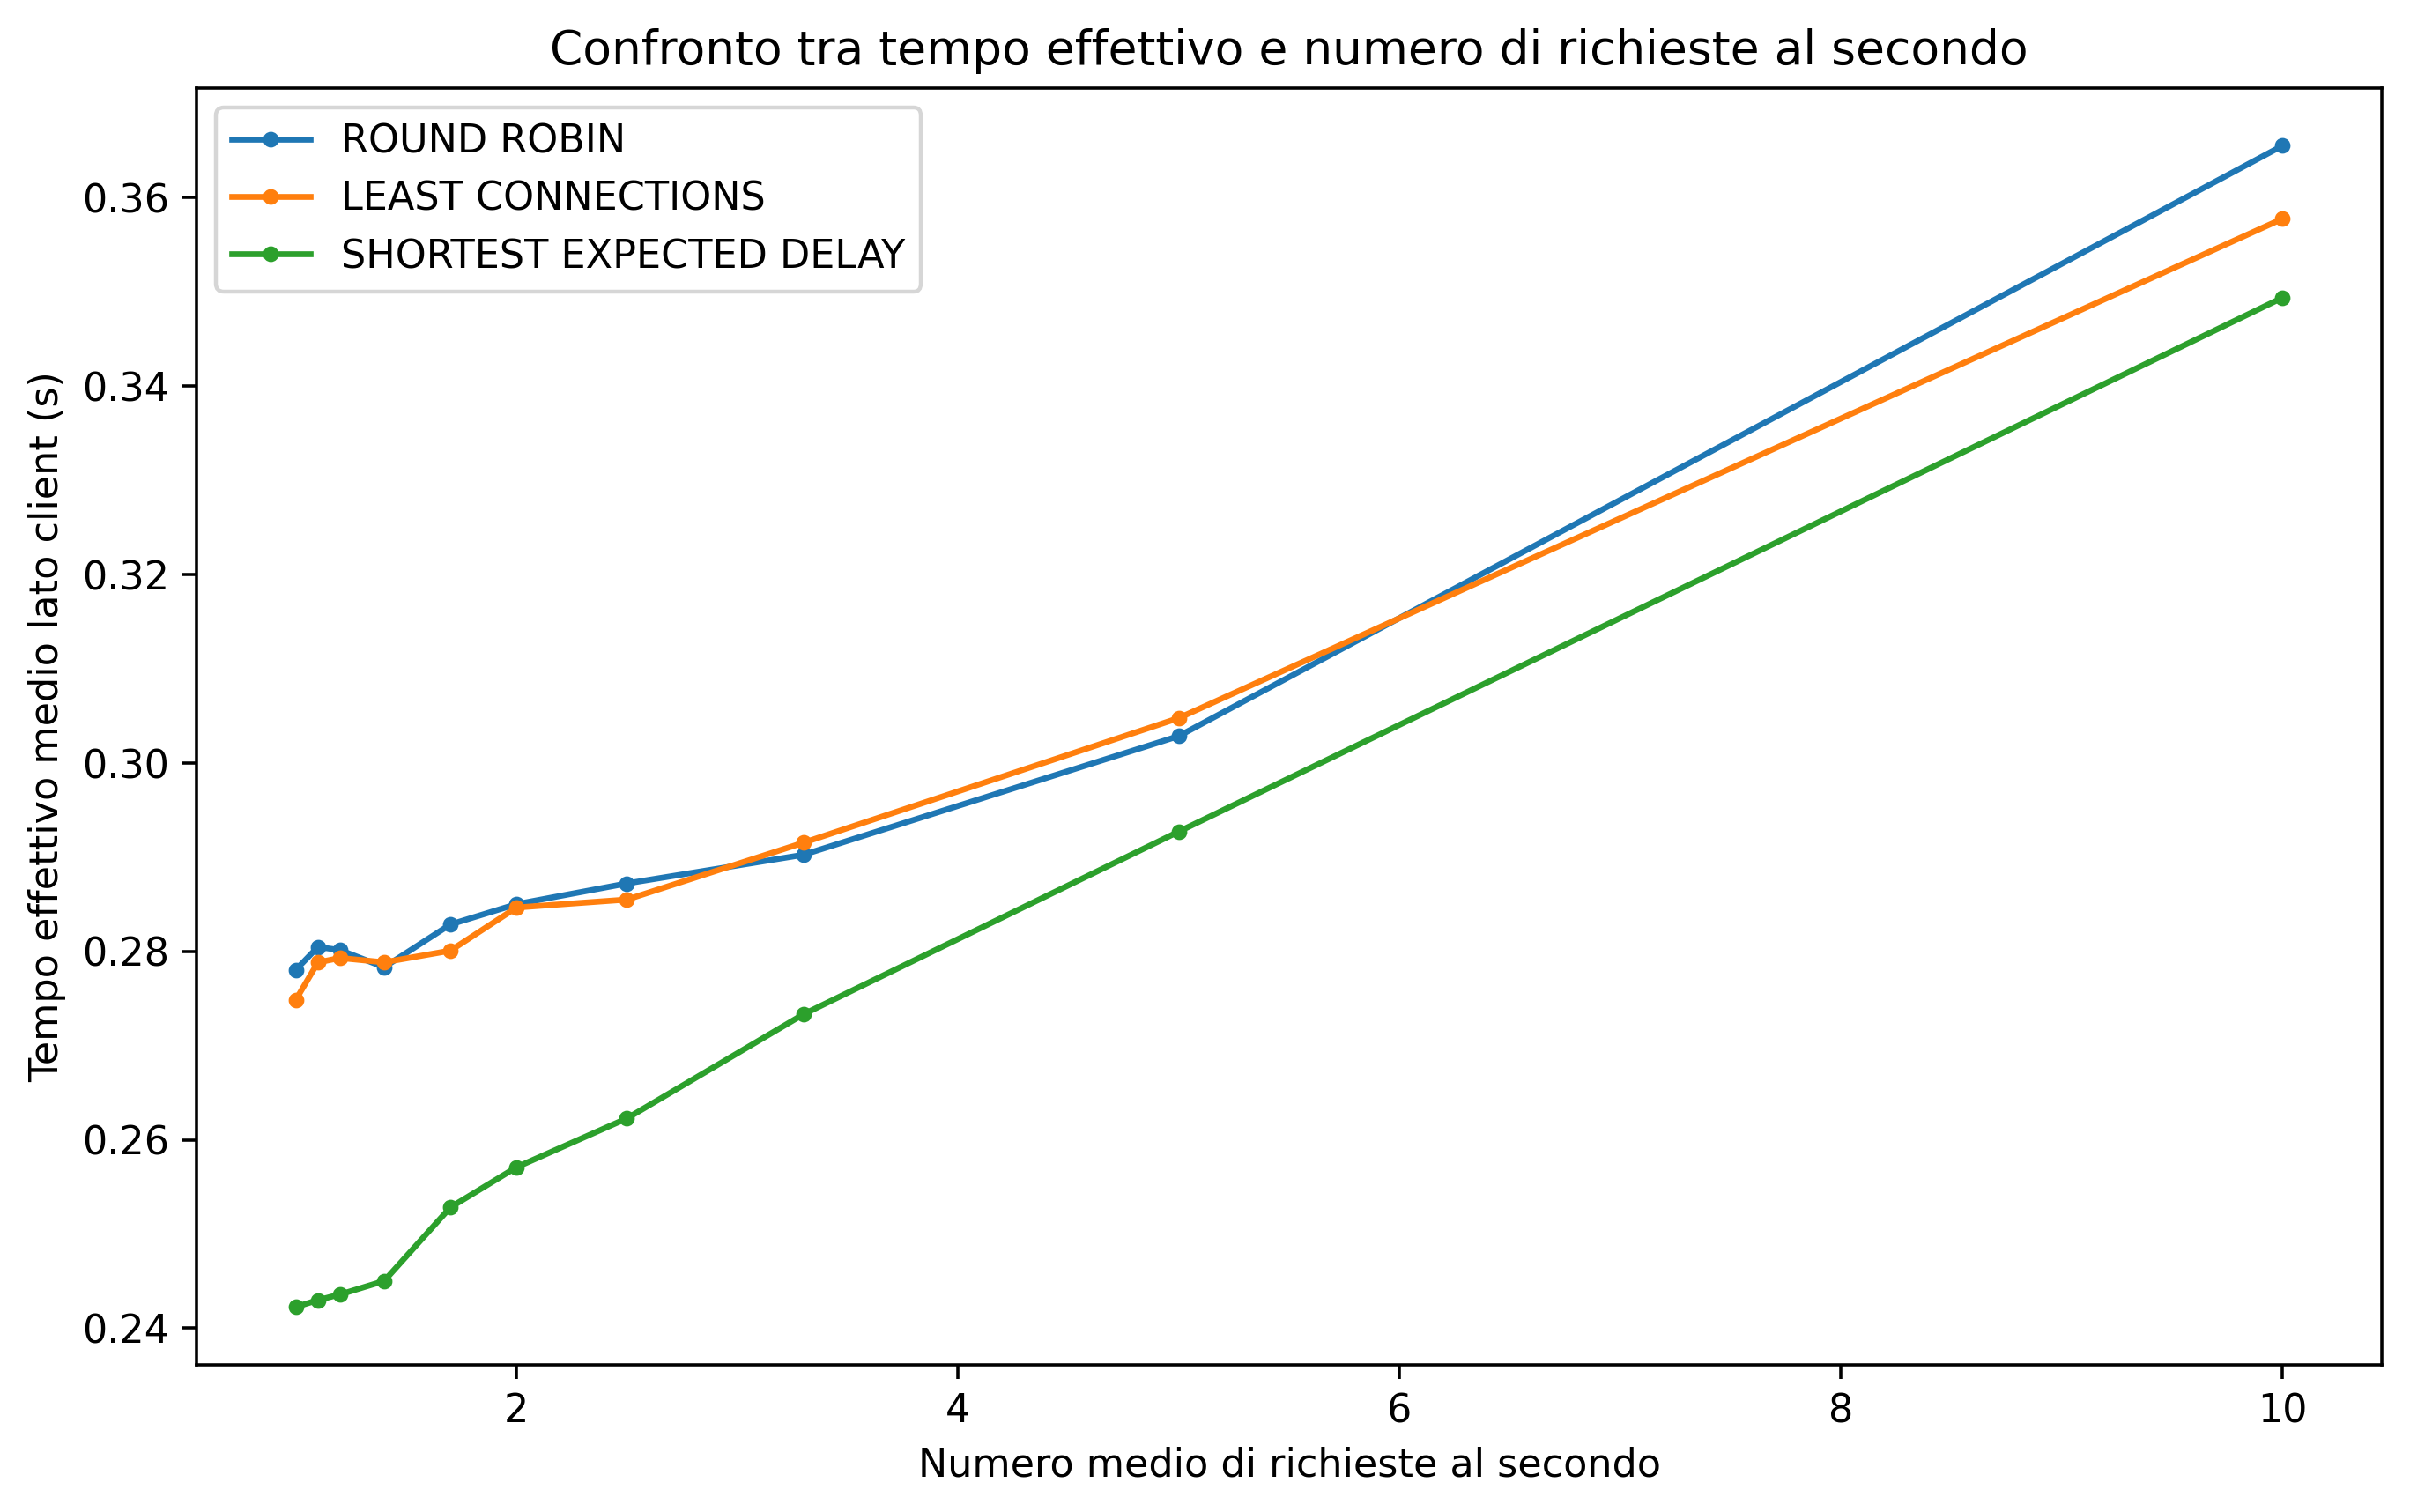
\includegraphics[width=\linewidth]{14_grafico_rtt.png}
    \caption{Confronto tra il RTT e il numero di richieste al secondo.}
    \label{fig:grafico-rtt}
\end{figure}

Come possiamo notare in \figurename~\ref{fig:grafico-rtt} al crescere dell'intensità delle richieste aumenta anche il tempo impiegato per elaborarle: questo effetto è normale in un'architettura come la nostra dove il server occupa tempo di CPI per simulare l'elaborazione delle richieste.

Gli scheduler rispettano tutti questa condizione, tuttavia l'algoritmo \textit{shortest expected delay} porta risultati migliori, soprattutto quando il numero di richieste è inferiore. Osservando il grafico in \figurename~\ref{fig:grafico-scheduler} potremo notare che gli altri scheduler ripartiscono equamente le richieste tra i nodi, aumentando quelle assegnate al \texttt{node-b}. Ricordandoci che il \texttt{node-b} ha un link con delay maggiore possiamo dedurre che questo porti il RTT medio ad aumentare.

Possiamo quindi affermare che l'algoritmo \textit{shortest expected delay} nella nostra architettura sia da preferire in tutti i casi analizzati, in quanto tiene in considerazione il delay sul \texttt{node-b}. Gli algoritmi \textit{Round-Robin} e \textit{least connections} sono invece più indicati in ambiti dove i nodi sono collocati nella stessa area geografica, in quanto sono più performanti all'aumentare delle richieste.

\section{Selezione dei nodi}

Vogliamo ora analizzare come cambia la distribuzione delle richieste ai vari nodi all'aumentare del numero di richieste. Osservare il comportamento dei vari scheduler ci permetterà di capire se considerano il delay sul link che collega il nodo, preferendo quindi tali scheduler in situazioni geograficamente distribuite.

Abbiamo quindi analizzato per ogni scheduler la percentuale di richieste che viene assegnata al \texttt{node-b}, ovvero quello con link con delay maggiore, all'aumentare delle stesse. Osserveremo così se lo scheduler tiene conto del delay sul nodo o meno e come questo comportamento vari all'aumento del tempo di gestione della richiesta sul nodo con link con delay minore. 

Ci aspettiamo che gli scheduler che tengono conto del ritardo sul link inoltrino poche richieste al nodo più distante quando il loro numero è basso e aumentino la percentuale al crescere dell'intensità. Questo accade in virtù del concetto di competitività descritto nei capitoli precedenti: il delay minore è compensato dalla congestione di richieste, che porta i nodi ad essere ugualmente competitivi.

\begin{figure}[H]
    \centering
    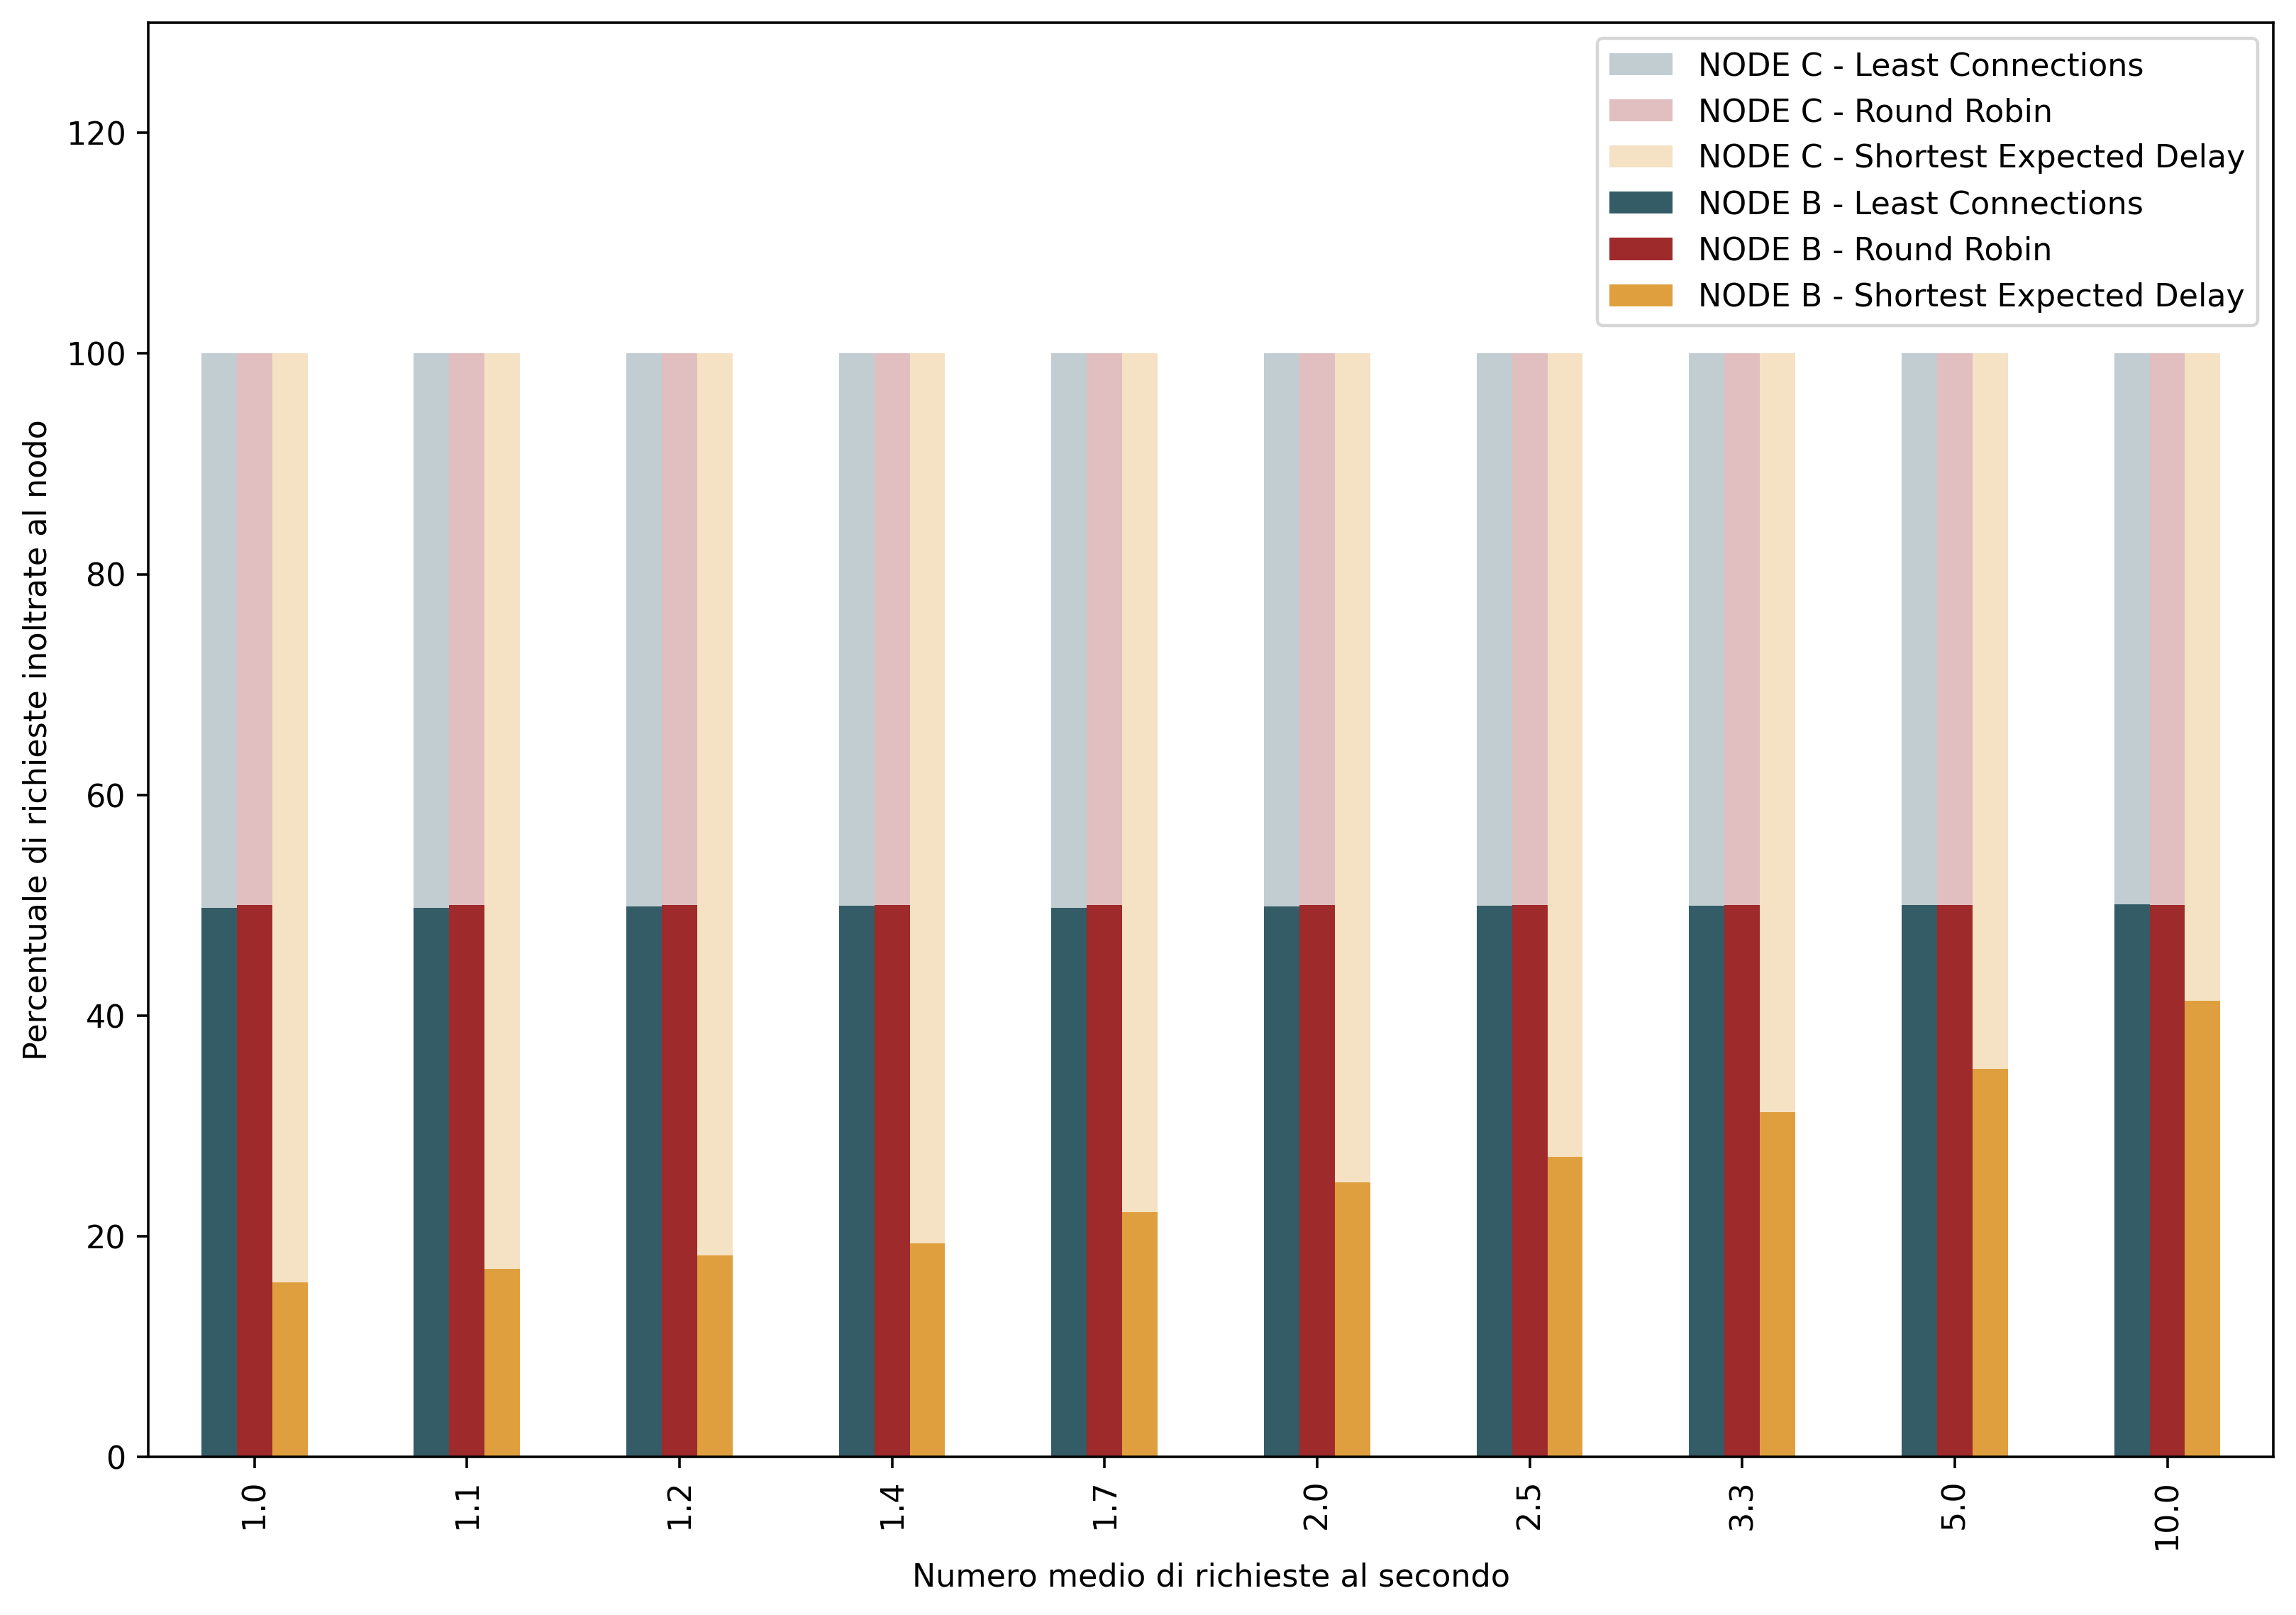
\includegraphics[width=\linewidth]{15_grafico_scheduler.png}
    \caption{Distribuzione delle richieste sui nodi tra i vari scheduler}
    \label{fig:grafico-scheduler}
\end{figure}

Come possiamo notare in \figurename~\ref{fig:grafico-scheduler} sono presenti due gruppi di algoritmi di scheduling:

\begin{itemize}
    \item gli scheduler che non tengono in considerazione il delay maggiore sul \texttt{node-b} e quindi ripartiscono equamente le richieste sui nodi. A questa categoria appartengono gli scheduler \textit{least connections} e \textit{round-robin}. La percentuale di richieste inoltrate rimane uguale all'aumentare dell'intensità in quanto i nodi hanno già una competitività bilanciata.
    \item gli scheduler che tengono invece in considerazione il delay sul link del nodo, dove notiamo solo lo scheduler \textit{shortest expected delay}. In questo caso la competitività è in favore del \texttt{node-c}, con delay maggiore, a cui vengono inizialmente assegnate la maggior parte delle richieste. All'aumentare dell'intensità la competitività viene bilanciata dalla congestione sul nodo con link con delay minore, che porta il sistema in una situazione di equilibrio.
\end{itemize}

Possiamo affermare come lo scheduler \textit{shortest expected delay} sia il più efficiente per quanto riguarda la nostra architettura in quanto porta la maggior parte delle richieste sul nodo con link con delay minore. È importante notare come questo non sia vero nel caso in cui l'intensità sia molto alta, tale da vanificare il vantaggio geografico, dove uno scheduler appartenente al primo gruppo risulta più performante. Come abbiamo affermato in precedenza, inoltre, queste considerazioni non valgono nel caso i nodi presentino un delay sul link equiparabile dove la scelta di uno scheduler che tiene in conto del ritardo sul link porta un'inutile overhead computazionale sul nodo a cui si fa inizialmente richiesta. 

\chapter*{Conclusioni}
\addcontentsline{toc}{chapter}{Conclusioni}  

%\section*{Raggiungimento degli obiettivi}
In questo lavoro di tesi abbiamo creato un ambiente di emulazione di architetture di edge computing composto da sistemi flessibili e con un'ampia adozione da parte delle realtà del settore, sfruttando KVM e Kubernetes. La scelta di queste due tecnologie permette una grande flessibilità e una notevole estendibilità, come abbiamo più volte evidenziato nei capitoli precedenti.

È importante rimarcare anche la grande personalizzazione che deriva dalla progettazione della parte di networking. Nel nostro caso abbiamo introdotto un delay artificiale sui nodi, ma è possibile sfruttare il sistema operativo GNU/Linux per regolare al meglio l'emulazione degradando ulteriormente le caratteristiche di rete. 

L'introduzione del ritardo artificiale sui link della rete ci ha permesso di simulare la distanza geografica tra i nodi, consentendo l'analisi delle peculiarità e caratteristiche degli algoritmi di scheduling implementati da Kubernetes, nonché le relative performance. 

Sulla base dei risultati dei test e dai dati raccolti possiamo affermare che in un ambiente geograficamente distribuito l'algoritmo \textit{shortest expected delay} è generalmente più performante. Al contrario gli algoritmi \textit{Round-Robin} e \textit{least connections} sono più indicati in realtà dove i nodi di computazione sono in una singola area geografica, in quanto a parità di richieste e delay tra nodi offrono prestazioni migliori.

Tuttavia, è importante notare come l'ambiente consenta l'analisi di una qualsiasi configurazione di rete e algoritmo di scheduling. Questo è un risultato molto importante che mostra la grande flessibilità dell'ambiente di emulazione progettato e implementato.

\section*{Sviluppi futuri}

In questa sezione vedremo alcune idee sulle possibili evoluzioni del progetto. È molto importante notare come queste dipendano dalle tecnologie disponibili e da possibili evoluzioni di queste.

\subsection*{Simu5G}

Un'importante evoluzione sarebbe data dall'uso del sistema di simulazione \texttt{OMNeT++} e del suo framework \texttt{Simu5G}. Grazie a questi sarebbe possibile generare le richieste da \textit{user equipment} simulati verso l'applicazione reale, permettendo di considerare nella simulazione anche la rete 5G. 

Potremmo poi simulare lo spostamento dei vari \textit{user equipment} nello spazio virtuale, cambiando la sua locazione geografica e portando a una ridefinizione dei nodi più competitivi. Questo porterebbe a un'analisi più completa del sistema di emulazione soprattutto per quanto riguarda la parte di selezione \textit{on the fly} del nodo più competitivo.

\subsection*{Uso di componenti fisici}

Un filo evolutivo che è utile tenere in considerazione consiste nella progressiva trasformazione delle componenti emulate o virtuali in componenti hardware: le macchine virtuali potrebbero diventare macchine fisiche e la parte di emulazione della rete 5G potrebbe passare attraverso componenti ugualmente fisiche.
Nonostante il costo per nulla indifferente potremmo analizzare con più attenzione ai particolari la bontà del sistema e capire maggiormente le implicazioni che gli scheduler hanno sulla scelta del nodo più competitivo.

\bibliographystyle{ieeetr}
\bibliography{biblio}

\newgeometry{top=3.5cm}

\chapter*{Ringraziamenti}
\addcontentsline{toc}{chapter}{Ringraziamenti}  

Vorrei dedicare questo spazio per esprimere la mia più sincera gratitudine verso quelle persone che sono state, e sono tuttora, importanti nella mia vita. 

Prima, tuttavia, vorrei ringraziare il mio relatore, Christian, che con disponibilità e pazienza mi ha accompagnato lungo il mio percorso. Gran parte di questo lavoro non sarebbe mai stato possibile senza lui.

Vorrei ringraziare Anna, la mia compagna, che in tutti questi anni non ha mai smesso di supportarmi (e \textit{sopportarmi}): ci sei sempre stata, sia nei momenti migliori che in quelli peggiori, e il tuo sostegno mi ha aiutato ad affrontare ogni sfida con fiducia e determinazione. Di questo ti sono immensamente grato. Grazie per esserci e per essere ciò che sei.

Ci tengo a menzionare i miei amici, mio fratello e tutti coloro con cui ho condiviso momenti felici e spensierati. Ho scherzato, ho riso, ho giocato e ho pianto con voi. Vi ringrazio per ciò che siete e per la parte importante che rappresentate nella mia vita, senza di voi il percorso che mi ha portato fino a qua non sarebbe stato altrettanto intenso ed emozionante.

Non potrei concludere senza citare i miei genitori: i vostri insegnamenti (anche quando non li ho ascoltati) sono stati preziosi, così come lo è stato il vostro supporto durante tutti questi anni. È difficile descrivere in qualche parola la mia profonda gratitudine per tutti gli sforzi e i sacrifici che avete fatto, e che fate tuttora, per darmi tutte le opportunità che ho avuto. Grazie per avermi fatto diventare ciò che sono.

\restoregeometry

\end{document}
